% Options for packages loaded elsewhere
\PassOptionsToPackage{unicode}{hyperref}
\PassOptionsToPackage{hyphens}{url}
\PassOptionsToPackage{dvipsnames,svgnames,x11names}{xcolor}
%
\documentclass[
  11pt,
]{article}
\usepackage{amsmath,amssymb}
\usepackage{iftex}
\ifPDFTeX
  \usepackage[T1]{fontenc}
  \usepackage[utf8]{inputenc}
  \usepackage{textcomp} % provide euro and other symbols
\else % if luatex or xetex
  \usepackage{unicode-math} % this also loads fontspec
  \defaultfontfeatures{Scale=MatchLowercase}
  \defaultfontfeatures[\rmfamily]{Ligatures=TeX,Scale=1}
\fi
\usepackage{lmodern}
\ifPDFTeX\else
  % xetex/luatex font selection
\fi
% Use upquote if available, for straight quotes in verbatim environments
\IfFileExists{upquote.sty}{\usepackage{upquote}}{}
\IfFileExists{microtype.sty}{% use microtype if available
  \usepackage[]{microtype}
  \UseMicrotypeSet[protrusion]{basicmath} % disable protrusion for tt fonts
}{}
\makeatletter
\@ifundefined{KOMAClassName}{% if non-KOMA class
  \IfFileExists{parskip.sty}{%
    \usepackage{parskip}
  }{% else
    \setlength{\parindent}{0pt}
    \setlength{\parskip}{6pt plus 2pt minus 1pt}}
}{% if KOMA class
  \KOMAoptions{parskip=half}}
\makeatother
\usepackage{xcolor}
\usepackage[margin=2.3cm]{geometry}
\usepackage{longtable,booktabs,array}
\usepackage{calc} % for calculating minipage widths
% Correct order of tables after \paragraph or \subparagraph
\usepackage{etoolbox}
\makeatletter
\patchcmd\longtable{\par}{\if@noskipsec\mbox{}\fi\par}{}{}
\makeatother
% Allow footnotes in longtable head/foot
\IfFileExists{footnotehyper.sty}{\usepackage{footnotehyper}}{\usepackage{footnote}}
\makesavenoteenv{longtable}
\usepackage{graphicx}
\makeatletter
\def\maxwidth{\ifdim\Gin@nat@width>\linewidth\linewidth\else\Gin@nat@width\fi}
\def\maxheight{\ifdim\Gin@nat@height>\textheight\textheight\else\Gin@nat@height\fi}
\makeatother
% Scale images if necessary, so that they will not overflow the page
% margins by default, and it is still possible to overwrite the defaults
% using explicit options in \includegraphics[width, height, ...]{}
\setkeys{Gin}{width=\maxwidth,height=\maxheight,keepaspectratio}
% Set default figure placement to htbp
\makeatletter
\def\fps@figure{htbp}
\makeatother
\setlength{\emergencystretch}{3em} % prevent overfull lines
\providecommand{\tightlist}{%
  \setlength{\itemsep}{0pt}\setlength{\parskip}{0pt}}
\setcounter{secnumdepth}{-\maxdimen} % remove section numbering
\ifLuaTeX
\usepackage[bidi=basic]{babel}
\else
\usepackage[bidi=default]{babel}
\fi
\babelprovide[main,import]{spanish}
% get rid of language-specific shorthands (see #6817):
\let\LanguageShortHands\languageshorthands
\def\languageshorthands#1{}
\usepackage{fontspec}
\setmonofont{DejaVu Sans Mono}[Scale=0.82]
\usepackage{tikz}
\usetikzlibrary{arrows.meta,positioning}
\usepackage{booktabs,float,caption,fancyhdr,etoolbox,xurl,graphicx}
\usepackage{enumitem}
\setlist{itemsep=2pt,topsep=4pt}
\pagestyle{fancy}\fancyhf{}
\fancyhead[L]{\small CC3069 --- Proyecto 3: Mejorando algoritmos con CUDA}
\fancyfoot[C]{\thepage}
\renewcommand{\headrulewidth}{0.3pt}
\setlength{\headheight}{14pt}
\captionsetup{font=small,labelfont=bf}
\AtBeginEnvironment{longtable}{\small}
\setlength{\LTpre}{8pt}\setlength{\LTpost}{8pt}
\setlength{\emergencystretch}{3em}
\usepackage{fvextra}
\DefineVerbatimEnvironment{verbatim}{Verbatim}{fontsize=\scriptsize,breaklines=true,breakanywhere=true}
\usepackage{newunicodechar}
\newunicodechar{≈}{\ensuremath{\approx}}
\sloppy
\ifLuaTeX
  \usepackage{selnolig}  % disable illegal ligatures
\fi
\usepackage{bookmark}
\IfFileExists{xurl.sty}{\usepackage{xurl}}{} % add URL line breaks if available
\urlstyle{same}
\hypersetup{
  pdftitle={Informe Final: Proyecto 3 --- Mejorando Algoritmos con CUDA},
  pdfauthor={CC3069 Computación Paralela y Distribuida · UVG · Semestre II 2026},
  pdflang={es},
  colorlinks=true,
  linkcolor={black},
  filecolor={Maroon},
  citecolor={Blue},
  urlcolor={blue},
  pdfcreator={LaTeX via pandoc}}

\title{Informe Final: Proyecto 3 --- Mejorando Algoritmos
con CUDA}
\usepackage{etoolbox}
\makeatletter
\providecommand{\subtitle}[1]{% add subtitle to \maketitle
  \apptocmd{\@title}{\par {\large #1 \par}}{}{}
}
\makeatother
\subtitle{Aceleración del entrenamiento de redes
convolucionales para clasificación de lenguaje de señas (ASL
Alphabet)}
\author{José Mérida (201101)\\ Javier España (23361)\\ Angel Esquit (23221)\\[4mm]
CC3069 Computación Paralela y Distribuida · UVG · Semestre II 2026}
\date{Noviembre 2026}

\begin{document}
\begin{titlepage}
\centering
\vspace*{1cm}
{\Large\bfseries Universidad del Valle de Guatemala\par}
\vspace{2mm}
{\large Facultad de Ingeniería\par}
{\large Departamento de Ciencias de la Computación\par}
\vspace{8mm}
{\large CC3069 --- Computación Paralela y Distribuida\par}
{\large Semestre II 2026\par}
\vfill
{\huge\bfseries Proyecto 3\par}
\vspace{4mm}
{\LARGE Mejorando algoritmos con CUDA\par}
\vspace{8mm}
{\large Aceleración del entrenamiento de redes convolucionales\\
para el reconocimiento de lenguaje de señas (ASL Alphabet)\par}
\vfill
{\large\bfseries Integrantes\par}
\vspace{3mm}
{\large
José Mérida \quad 201101\\[1mm]
Javier España \quad 23361\\[1mm]
Angel Esquit \quad 23221\par}
\vspace{2cm}
{\large Guatemala, noviembre de 2026\par}
\end{titlepage}
\setcounter{page}{2}
\clearpage
\tableofcontents
\clearpage

\clearpage
\section*{Entorno de Hardware y Software}
\addcontentsline{toc}{section}{Entorno de Hardware y Software}

\begin{itemize}
\tightlist
\item
  \textbf{CPU:} Intel(R) Core(TM) i5-14600KF, 20 hilos
  lógicos
\item
  \textbf{GPU:} NVIDIA GeForce RTX 4070 SUPER (12,282 MiB
  VRAM, arquitectura Ada Lovelace), en todos los benchmarks
  y en el entrenamiento completo de la sección 5.4.
\item
  \textbf{Host-Device Interconnect:} PCI Express 4.0 x16
\item
  \textbf{Software Stack:} Python 3.13, PyTorch 2.9.1+cu128,
  CUDA Toolkit 12.9 / driver 580.95 (CUDA 13.0), CuPy 14.2.0
  (\texttt{cupy-cuda12x}), TensorFlow 2.18, NumPy 2.2.6
\end{itemize}

\section{Resumen Ejecutivo}\label{resumen-ejecutivo}

El presente proyecto aborda la aceleración computacional del
entrenamiento de tres arquitecturas de Redes Neuronales
Convolucionales (CNN-1 Baseline, CNN-2 Profunda y CNN-3
Regularizada con Batch Normalization y Dropout) aplicadas a
la clasificación de 29 gestos del alfabeto de Lenguaje de
Señas Americano (ASL Alphabet, 14,500 imágenes 64x64x3).
Partiendo de la implementación secuencial en CPU del
Laboratorio 3 de Data Science, se aplicó un rediseño
arquitectónico paralelo cumpliendo rigurosamente la
directriz de la cátedra: \textbf{la preparación y
decodificación de datos se ejecuta exclusivamente en CPU
multinúcleo, reservando la GPU para la matemática tensorial
intensiva (propagación hacia adelante, retropropagación y
optimización de parámetros)}.

Se implementaron y compararon seis entornos de ejecución
sobre los mismos datos y particiones:

\begin{enumerate}
\def\labelenumi{\arabic{enumi}.}
\tightlist
\item
  \textbf{Keras / TensorFlow en CPU:} Línea base secuencial
  original.
\item
  \textbf{PyTorch en CPU:} Control en CPU bajo un framework
  tensorial moderno.
\item
  \textbf{NumPy en CPU (Desde Cero):} Implementación
  algorítmica pura con \texttt{im2col} matricial en CPU.
\item
  \textbf{CuPy en GPU (Desde Cero):} Implementación
  algorítmica idéntica en GPU, solo con operaciones de CuPy
  y cuBLAS.
\item
  \textbf{CuPy en GPU con kernels CUDA propios:} La misma
  red, con \texttt{im2col}, \texttt{col2im}, ReLU, MaxPool y
  Adam escritos como \texttt{cp.RawKernel} (CUDA C).
\item
  \textbf{PyTorch en GPU (CUDA + cuDNN):} Solución acelerada
  de alto rendimiento.
\end{enumerate}

Los resultados experimentales demuestran un \textbf{speedup
de hasta 14.9x en PyTorch CUDA frente a Keras CPU}, un
\textbf{speedup de hasta 24.4x frente a PyTorch CPU}, y, en
la comparación desde cero con el mismo algoritmo,
\textbf{58.9x de CuPy frente a NumPy} (\textbf{92.9x} con
kernels CUDA propios). Los kernels propios aceleran la época
1.58x en CNN-1 pero solo 1.11x a 1.12x en CNN-2 y CNN-3,
donde domina la multiplicación de matrices en cuBLAS;
ninguna variante desde cero alcanza a PyTorch + cuDNN (1.6x
a 2.9x más lento). El análisis con la Ley de Amdahl muestra
que la fracción no acelerable medida (armado del lote en CPU
y transferencia H2D, 0.081 s por época en CNN-3) es solo el
0.36 \% del tiempo secuencial, así que el speedup no lo
limita la parte serial sino la aceleración efectiva de la
GPU sobre la parte paralela (15.7x). Los modelos entrenados
en GPU convergieron con Early Stopping a \textbf{99.59 \% de
exactitud en CNN-2} y \textbf{99.31 \% en CNN-3}.

\clearpage
\section*{Evidencia de Ejecución: CPU en la fase de datos, GPU en el entrenamiento}
\addcontentsline{toc}{section}{Evidencia de Ejecución: CPU en la fase de datos, GPU en el entrenamiento}

Capturas reales de la terminal (\texttt{nvidia-smi} y \texttt{top} por núcleo) en la RTX 4070 SUPER, tomadas con
\texttt{scripts/capture\_evidence.sh} mientras corría cada fase. Los recuadros amarillos y las notas se
agregaron encima de la captura original (sin tocar los números); los textos originales están en
\texttt{results/evidence/screens/}.

\begin{center}
\renewcommand{\arraystretch}{1.6}
\begin{tabular}{|p{0.26\textwidth}|c|c|p{0.30\textwidth}|}
\hline
\textbf{Fase} & \textbf{GPU (uso)} & \textbf{GPU (proceso CUDA)} & \textbf{CPU} \\
\hline
\textbf{A. Preparación de datos} & \textbf{4 \%} (31 W) & \textbf{ninguno} & \textbf{20 hilos} al 45--67 \%, 20 procesos \texttt{pt\_data\_worker} \\
\hline
\textbf{B. Entrenamiento CUDA} & \textbf{96 \%} (183 W) & \textbf{\texttt{python3}, tipo C, 836 MiB} & hilos de PyTorch y el lanzador de kernels \\
\hline
\end{tabular}
\end{center}

\textbf{Qué demuestran:} (1) mientras se leen y decodifican las imágenes la GPU está prácticamente ociosa
y trabaja la CPU con todos sus hilos; (2) cuando empieza el entrenamiento la GPU salta a 96 \% y aparece un
proceso de cómputo CUDA en ella. Es decir, la preparación de archivos corre en CPU y la matemática de la red en GPU.

\begin{center}
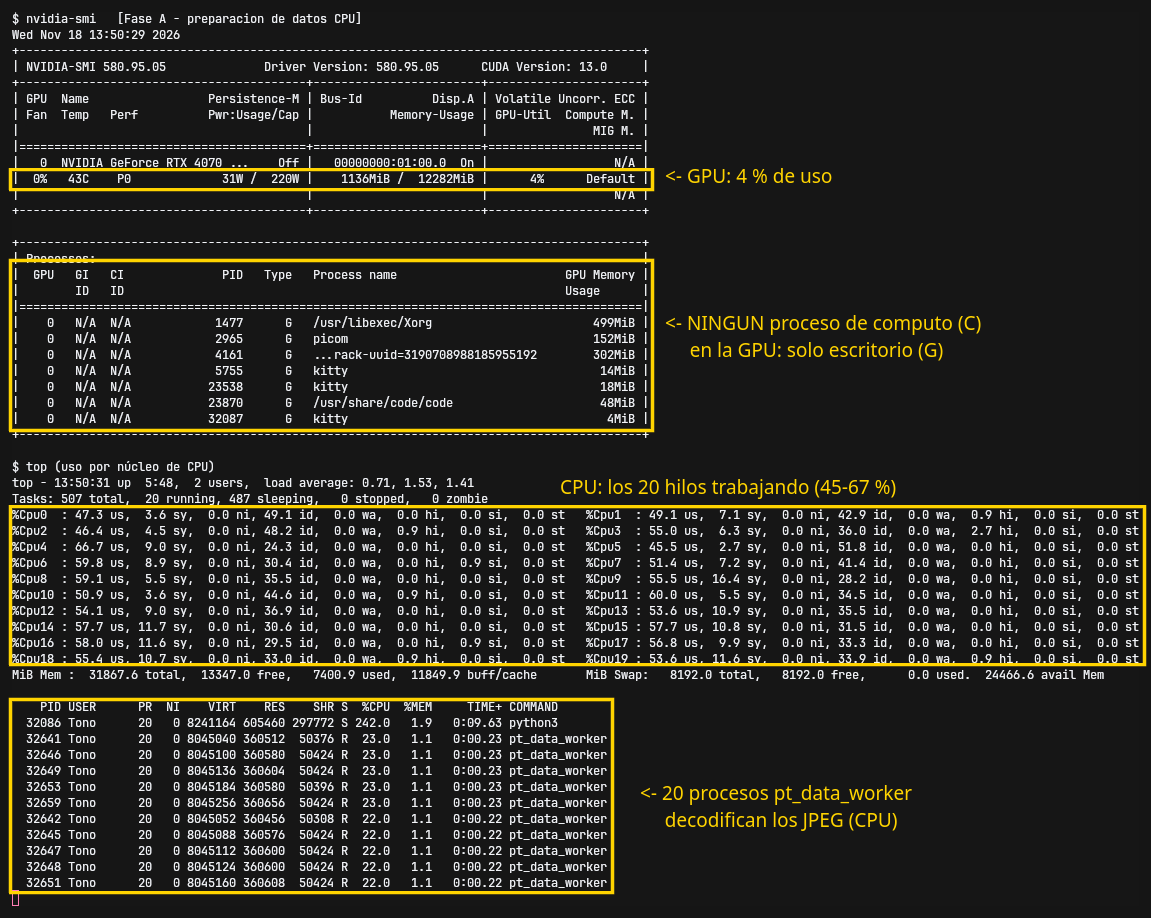
\includegraphics[width=\textwidth]{../results/evidence/screens/2_datos_cpu_anotada.png}\\
\emph{Figura A: Fase A, preparación de datos. GPU al 4 \%, sin proceso de cómputo (solo procesos gráficos \texttt{G}); CPU con 20 hilos ocupados.}
\end{center}

\clearpage
\begin{center}
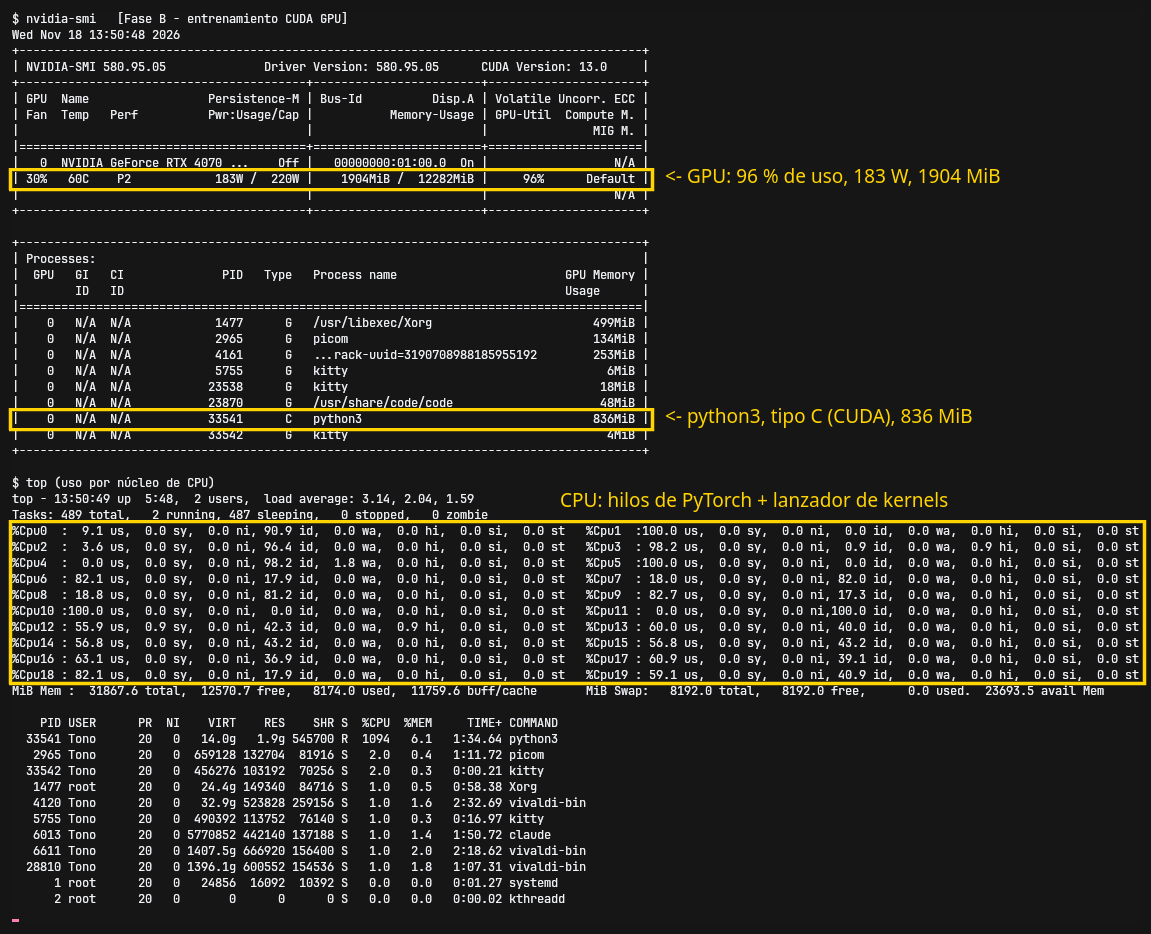
\includegraphics[width=\textwidth]{../results/evidence/screens/3_entrenamiento_gpu_anotada.png}\\
\emph{Figura B: Fase B, entrenamiento en CUDA. GPU al 96 \% (183 W de 220 W, 1,904 MiB de VRAM); \texttt{python3} aparece con tipo \texttt{C} (cómputo) usando 836 MiB.}
\end{center}

La captura en reposo (\texttt{1\_reposo.png}) y las gráficas de tiempo (sección 5.5) completan la evidencia.

\clearpage
\section{1. Análisis del Algoritmo Secuencial (Paso
1)}\label{anuxe1lisis-del-algoritmo-secuencial-paso-1}

\subsection{1.1 Descripción del Algoritmo y Flujo de
Trabajo}\label{descripciuxf3n-del-algoritmo-y-flujo-de-trabajo}

El problema original consiste en clasificar imágenes en
color de 64x64 píxeles en 29 categorías (26 letras de la `A'
a la `Z', más `del', `nothing' y `space'). El dataset consta
de 14,500 muestras particionadas estratificadamente en:

\begin{itemize}
\tightlist
\item
  \textbf{Entrenamiento:} 11,600 imágenes (80\%)
\item
  \textbf{Validación:} 1,450 imágenes (10\%)
\item
  \textbf{Prueba:} 1,450 imágenes (10\%)
\end{itemize}

El algoritmo secuencial original (ejecutado en
\texttt{notebooks/01\_baseline\_keras.ipynb}) procesa estas
imágenes en un pipeline lineal dividido en 12 operaciones
fundamentales:

\begin{longtable}[]{@{}
  >{\centering\arraybackslash}p{(\columnwidth - 8\tabcolsep) * \real{0.0659}}
  >{\raggedright\arraybackslash}p{(\columnwidth - 8\tabcolsep) * \real{0.1758}}
  >{\raggedright\arraybackslash}p{(\columnwidth - 8\tabcolsep) * \real{0.4505}}
  >{\centering\arraybackslash}p{(\columnwidth - 8\tabcolsep) * \real{0.1209}}
  >{\centering\arraybackslash}p{(\columnwidth - 8\tabcolsep) * \real{0.1868}}@{}}
\toprule\noalign{}
\begin{minipage}[b]{\linewidth}\centering
No.
\end{minipage} & \begin{minipage}[b]{\linewidth}\raggedright
Operación
\end{minipage} & \begin{minipage}[b]{\linewidth}\raggedright
Descripción Técnica
\end{minipage} & \begin{minipage}[b]{\linewidth}\centering
Ubicación
\end{minipage} & \begin{minipage}[b]{\linewidth}\centering
Intensidad de Cómputo
\end{minipage} \\
\midrule\noalign{}
\endhead
\bottomrule\noalign{}
\endlastfoot
1 & Lectura de splits & Carga de archivos CSV con rutas
relativas y etiquetas string & CPU & Muy Baja (I/O texto) \\
2 & Lectura de archivos & \texttt{read\_file}: carga
secuencial de bytes JPEG desde disco & CPU & Media (I/O
binario) \\
3 & Decodificación JPEG & Descompresión de imagen JPEG a
matriz numérica \texttt{uint8} & CPU & Media
(Entropía/Huffman) \\
4 & Redimensionado & Interpolación bilineal/bicúbica a
dimensiones 64x64 & CPU & Media \\
5 & Normalización y One-Hot & Conversión a flotante
\([0, 1]\) (\texttt{float32}) y vector de 29 clases & CPU &
Baja \\
6 & Batching y Shuffle & Conformación de tensores de lote de
dimensión \((64, 64, 64, 3)\) & CPU & Baja (Indexado en
RAM) \\
7 & \textbf{Forward de la Red} & Convolución 2D, activación
ReLU, MaxPool, BatchNorm, FC & \textbf{GPU (Candidata)} &
\textbf{Extremadamente Alta} \\
8 & \textbf{Cálculo de Pérdida} & Softmax y Categorical
Cross-Entropy sobre 29 logits & \textbf{GPU (Candidata)} &
\textbf{Alta} \\
9 & \textbf{Backward (Gradientes)} & Regla de la cadena
retropropagada en todas las capas & \textbf{GPU (Candidata)}
& \textbf{Extremadamente Alta} \\
10 & \textbf{Optimizador (Adam)} & Cálculo de momentos
\(m_t\), \(v_t\) y actualización de pesos & \textbf{GPU
(Candidata)} & \textbf{Alta} \\
11 & Control de Época & Evaluación en validación, Early
Stopping, ReduceLROnPlateau & CPU / GPU & Media \\
12 & Evaluación Final & Inferencia en prueba, cálculo de
métricas (Accuracy, Macro F1) & CPU / GPU & Media \\
\end{longtable}

\subsection{1.2 Identificación de Operaciones Repetitivas e
Intensivas}\label{identificaciuxf3n-de-operaciones-repetitivas-e-intensivas}

Durante cada época de entrenamiento se iteran 182 lotes de
tamaño 64. La tabla siguiente sintetiza las repeticiones
computacionales:

\begin{longtable}[]{@{}
  >{\raggedright\arraybackslash}p{(\columnwidth - 6\tabcolsep) * \real{0.2667}}
  >{\centering\arraybackslash}p{(\columnwidth - 6\tabcolsep) * \real{0.2778}}
  >{\centering\arraybackslash}p{(\columnwidth - 6\tabcolsep) * \real{0.2111}}
  >{\centering\arraybackslash}p{(\columnwidth - 6\tabcolsep) * \real{0.2444}}@{}}
\toprule\noalign{}
\begin{minipage}[b]{\linewidth}\raggedright
Operación Repetitiva
\end{minipage} & \begin{minipage}[b]{\linewidth}\centering
Tamaño de Datos por Ejecución
\end{minipage} & \begin{minipage}[b]{\linewidth}\centering
Repeticiones por Época
\end{minipage} & \begin{minipage}[b]{\linewidth}\centering
Repeticiones Totales (25 Épocas)
\end{minipage} \\
\midrule\noalign{}
\endhead
\bottomrule\noalign{}
\endlastfoot
Decodificación y normalización JPEG & 1 archivo imagen
(\textasciitilde10-30 KB) & 11,600 (única si hay caché) &
11,600 \\
Convolución 2D (Forward) & Tensor \((64, H, W, C_{in})\) &
\(182 \times (\text{capas})\) & 9,100 a 18,200 \\
Convolución 2D (Backward) & Tensor de gradientes de
activación & \(182 \times (\text{capas})\) & 9,100 a
18,200 \\
Actualización Adam & Todos los tensores de pesos y sesgos &
182 pasos & 4,550 actualizaciones \\
Inferencia en Validación & Lote de validación (23 lotes) &
23 pasos & 575 pasos \\
\end{longtable}

\subsection{1.3 Análisis de Complejidad y Operaciones MAC
(Multiply-Accumulate)}\label{anuxe1lisis-de-complejidad-y-operaciones-mac-multiply-accumulate}

La carga de trabajo matemática está dominada por las capas
convolucionales y completamente conectadas. Para una capa
convolucional 2D con entrada \((C_{in}, H_{in}, W_{in})\),
filtros de \(K \times K\) y \(C_{out}\) canales de salida,
el número de operaciones Multiply-Accumulate (MAC) por
imagen viene dado por:
\[\text{MACs}_{\text{Conv}} = H_{out} \times W_{out} \times C_{out} \times (C_{in} \times K^2)\]
Para una capa densa (Fully Connected) que conecta \(N_{in}\)
entradas con \(N_{out}\) salidas:
\[\text{MACs}_{\text{Dense}} = N_{in} \times N_{out}\]

Al evaluar cada una de las tres arquitecturas bajo análisis,
se obtienen las siguientes cifras teóricas por imagen:

\begin{longtable}[]{@{}
  >{\raggedright\arraybackslash}p{(\columnwidth - 10\tabcolsep) * \real{0.1250}}
  >{\raggedright\arraybackslash}p{(\columnwidth - 10\tabcolsep) * \real{0.3462}}
  >{\centering\arraybackslash}p{(\columnwidth - 10\tabcolsep) * \real{0.1250}}
  >{\centering\arraybackslash}p{(\columnwidth - 10\tabcolsep) * \real{0.1346}}
  >{\centering\arraybackslash}p{(\columnwidth - 10\tabcolsep) * \real{0.1346}}
  >{\centering\arraybackslash}p{(\columnwidth - 10\tabcolsep) * \real{0.1346}}@{}}
\toprule\noalign{}
\begin{minipage}[b]{\linewidth}\raggedright
Arquitectura
\end{minipage} & \begin{minipage}[b]{\linewidth}\raggedright
Capas Principales
\end{minipage} & \begin{minipage}[b]{\linewidth}\centering
Parámetros Totales
\end{minipage} & \begin{minipage}[b]{\linewidth}\centering
MACs Conv (por img)
\end{minipage} & \begin{minipage}[b]{\linewidth}\centering
MACs Dense (por img)
\end{minipage} & \begin{minipage}[b]{\linewidth}\centering
Total MACs / imagen
\end{minipage} \\
\midrule\noalign{}
\endhead
\bottomrule\noalign{}
\endlastfoot
\textbf{CNN-1 Baseline} & 2 Conv (32, 64) + Flatten +
Dense(64) + Dense(29) & \textbf{4,221,405} &
\textasciitilde22 M & \textasciitilde4.2 M &
\textbf{\textasciitilde26.2 M} \\
\textbf{CNN-2 Profunda} & 4 Conv (32, 64, 128, 128) + GAP +
Dense(64) + Dense(29) & \textbf{519,069} &
\textasciitilde158 M & \textasciitilde0.15 M &
\textbf{\textasciitilde158.2 M} \\
\textbf{CNN-3 Regularizada} & 4 Conv + BatchNorm + Dropout +
GAP + Dense + Dense & \textbf{448,925} & \textasciitilde171
M & \textasciitilde0.07 M & \textbf{\textasciitilde171.1
M} \\
\end{longtable}

\begin{quote}
\textbf{Hallazgo Fundamental de Arquitectura:}
\end{quote}

\begin{quote}
A pesar de que \textbf{CNN-1 tiene 8 veces más parámetros}
que CNN-2 y CNN-3 (debido a la capa de aplanado
\texttt{Flatten} hacia la capa densa con 4 millones de
conexiones), \textbf{CNN-2 y CNN-3 requieren
\textasciitilde7 veces más operaciones aritméticas (MACs)
por imagen} debido a la profundidad de los mapas de
características convolucionales. Esto explica con total
claridad por qué en la CPU secuencial CNN-2 y CNN-3 tardan
\textasciitilde22 segundos por época frente a los
\textasciitilde4 segundos de CNN-1.
\end{quote}

\clearpage
\section{2. Medición del Tiempo Secuencial (Paso
2)}\label{mediciuxf3n-del-tiempo-secuencial-paso-2}

\subsection{2.1 Protocolo Experimental de
Medición}\label{protocolo-experimental-de-mediciuxf3n}

Para aislar rigurosamente el \emph{throughput} computacional
y evitar sesgos estadísticos, se estableció el siguiente
protocolo:

\begin{enumerate}
\def\labelenumi{\arabic{enumi}.}
\tightlist
\item
  \textbf{Épocas fijas:} Se ejecutaron exactamente 5 épocas
  por modelo para benchmarks de velocidad, desactivando
  \texttt{EarlyStopping} para garantizar que todos los
  modelos procesen el mismo número exacto de lotes (182
  pasos por época \(\times\) 5 = 910 pasos).
\item
  \textbf{Repeticiones independientes:} 3 corridas completas
  por configuración (excepto PyTorch CPU, 1 corrida) para
  calcular media (\(\mu\)) y desviación estándar
  (\(\sigma\)). En las tablas, \(\sigma\) se calcula sobre
  las épocas 2 a 5 de todas las corridas.
\item
  \textbf{Descarte de calentamiento (Warm-up):} En la
  medición por época se excluye la primera época del cómputo
  promedio para evitar que la inicialización de buffers,
  compilación JIT y autotuning de cuDNN distorsionen los
  resultados.
\item
  \textbf{Sincronización:} En GPU se invocó explícitamente
  barreras de sincronización
  (\texttt{torch.cuda.synchronize()} en PyTorch y
  \texttt{Device().synchronize()} en CuPy) antes y después
  de cada bloque de medición para cronometrar el tiempo real
  de ejecución en hardware y no el tiempo asíncrono de
  encolamiento del host.
\end{enumerate}

\subsection{2.2 Tiempos Secuenciales en
CPU}\label{tiempos-secuenciales-en-cpu}

Se evaluaron tres variantes en CPU:

\begin{itemize}
\tightlist
\item
  \textbf{Keras CPU (TensorFlow 2.18):} Línea base
  secuencial original con operaciones C++ multihilo de
  Eigen/OpenMP.
\item
  \textbf{PyTorch CPU (2.9.1):} Mismo grafo de tensores en
  CPU.
\item
  \textbf{NumPy CPU:} Implementación algorítmica desde cero
  sin aceleración de hardware.
\end{itemize}

\begin{longtable}[]{@{}
  >{\raggedright\arraybackslash}p{(\columnwidth - 8\tabcolsep) * \real{0.1739}}
  >{\centering\arraybackslash}p{(\columnwidth - 8\tabcolsep) * \real{0.1848}}
  >{\centering\arraybackslash}p{(\columnwidth - 8\tabcolsep) * \real{0.2283}}
  >{\centering\arraybackslash}p{(\columnwidth - 8\tabcolsep) * \real{0.2283}}
  >{\centering\arraybackslash}p{(\columnwidth - 8\tabcolsep) * \real{0.1848}}@{}}
\toprule\noalign{}
\begin{minipage}[b]{\linewidth}\raggedright
Configuración
\end{minipage} & \begin{minipage}[b]{\linewidth}\centering
CNN-1 Baseline (s/época)
\end{minipage} & \begin{minipage}[b]{\linewidth}\centering
CNN-2 Profunda (s/época)
\end{minipage} & \begin{minipage}[b]{\linewidth}\centering
CNN-3 Regularizada (s/época)
\end{minipage} & \begin{minipage}[b]{\linewidth}\centering
Preparación de Datos (s)
\end{minipage} \\
\midrule\noalign{}
\endhead
\bottomrule\noalign{}
\endlastfoot
\textbf{Keras CPU (Línea Base)} & \(4.085 \pm 0.063\) s &
\(21.628 \pm 0.267\) s & \(22.496 \pm 0.342\) s &
\(0.440 \pm 0.010\) s \\
\textbf{PyTorch CPU} & \(9.583 \pm 1.110\) s &
\(36.168 \pm 1.256\) s & \(34.106 \pm 0.078\) s &
\(0.828 \pm 0.000\) s \\
\textbf{NumPy CPU (Desde Cero)} & \(64.123 \pm 7.809\) s &
\emph{(no medido, est. ≈ 280 a 350 s)} & \emph{(no medido,
est. ≈ 290 a 350 s)} & \(0.050\) s (RAM) \\
\end{longtable}

\begin{verbatim}
Comparativa de Tiempos Secuenciales (Segundos por Época en CPU):
======================================================================
Keras CPU:     [====] 4.08s (CNN-1)  |  [======================] 21.63s (CNN-2)  |  [=======================] 22.50s (CNN-3)
PyTorch CPU:   [=========] 9.58s     |  [====================================] 36.17s  |  [==================================] 34.11s
NumPy Scratch: [================================================================] 64.12s (CNN-1)
\end{verbatim}

\textbf{Análisis de las discrepancias en CPU:}\\
Keras/TensorFlow demostró ser más rápido en CPU que PyTorch
debido a que el runtime de TensorFlow compila internamente
grafos de ejecución de subgrafos convolucionales y optimiza
mejor el layout de memoria \texttt{NHWC} nativo en CPU,
reduciendo la sobrecarga de transposición de canales. Por su
parte, la implementación pura en NumPy con \texttt{im2col}
matricial en Python tardó 64.1 segundos por época en CNN-1
(CNN-2 y CNN-3 no se midieron: hacen \textasciitilde6x más
MACs por imagen. Estimación: la razón de tiempo CNN-2/CNN-1
en las configuraciones medidas es 3.5x a 5.3x, y 4.4x en
CuPy, que usa el mismo algoritmo \texttt{im2col}; aplicada a
los 64.1 s de NumPy da ≈ 280 a 340 s por época en CNN-2 y ≈
290 a 350 s en CNN-3, es decir, unos 25 a 30 min por corrida
de 5 épocas para cada modelo, y 2 a 2.5 h para un
entrenamiento de 25 épocas), evidenciando el elevado costo
computacional cuando no intervienen bibliotecas altamente
vectorizadas en C/C++ ni aceleradores paralelos.

\clearpage
\section{3. Oportunidades de Paralelización y Separación
CPU/GPU (Paso
3)}\label{oportunidades-de-paralelizaciuxf3n-y-separaciuxf3n-cpugpu-paso-3}

\emph{Cumplimiento estricto del criterio de evaluación (40\%
de la nota final)}

\subsection{3.1 Justificación Teórica de la Separación de
Roles}\label{justificaciuxf3n-teuxf3rica-de-la-separaciuxf3n-de-roles}

El enunciado del proyecto exige de forma taxativa:

\begin{quote}
\textbf{``Los archivos/imágenes se preparan en la CPU
(varios núcleos) y la GPU se usa solo para la matemática de
la red.''}
\end{quote}

La arquitectura de computación heterogénea CPU-GPU dicta
esta división por principios físicos y algorítmicos:

\begin{enumerate}
\def\labelenumi{\arabic{enumi}.}
\tightlist
\item
  \textbf{Por qué la preparación de datos NO debe ir en
  GPU:}

  \begin{itemize}
  \tightlist
  \item
    La decodificación JPEG es un proceso de descompresión
    con entropía de longitud variable (algoritmo de Huffman)
    que posee intrínsecamente dependencias secuenciales
    entre bits.
  \item
    Forzar la decodificación de archivos JPEG individuales
    en la GPU introduce divergencia de hilos (thread
    divergence) extrema en los warps de CUDA, desperdiciando
    el paralelismo SIMT.
  \item
    La lectura de archivos desde disco (I/O del sistema
    operativo) requiere llamadas al kernel del SO e
    interrupciones de almacenamiento, las cuales residen
    exclusivamente en el host (CPU).
  \item
    Utilizando la CPU multinúcleo con múltiples workers en
    paralelo (\texttt{DataLoader(num\_workers=20)} o
    decodificación paralela en hilos), la CPU puede
    descomprimir y preprocesar el siguiente lote mientras la
    GPU computa el lote actual.
  \end{itemize}
\item
  \textbf{Por qué la matemática de la red SÍ pertenece a la
  GPU:}

  \begin{itemize}
  \tightlist
  \item
    Las operaciones de convolución, multiplicación matricial
    (GEMM), activación ReLU y normalización por lotes son
    \textbf{``vergonzosamente paralelas'' (embarrassingly
    parallel)}: cada píxel del mapa de salida o cada neurona
    puede computarse de manera independiente.
  \item
    La GPU cuenta con miles de núcleos aritméticos y un
    ancho de banda de memoria GDDR6X de \textasciitilde500
    GB/s en la RTX 4070 SUPER (en contraste con los
    \textasciitilde40-60 GB/s de la memoria DDR5 del host).
  \end{itemize}
\end{enumerate}

\begin{center}
\resizebox{\textwidth}{!}{%
\begin{tikzpicture}[node distance=5mm and 7mm, box/.style={draw, rounded corners=2pt, align=center, font=\small, inner sep=4pt, minimum height=9mm, fill=#1}, box/.default=white, arr/.style={-{Stealth[length=2.2mm]}, thick}]
\node[box=gray!12] (d1) {Lectura de disco\\(SSD NVMe)};
\node[box=gray!12, right=of d1] (d2) {Decodificaci\'on JPEG\\en paralelo};
\node[box=gray!12, right=of d2] (d3) {Resize 64x64\\y normalizaci\'on};
\node[box=gray!12, right=of d3] (d4) {Lotes\\(64 im\'agenes)};
\node[box=gray!12, right=of d4] (d5) {Memoria\\paginable};
\node[box=green!15, below=14mm of d5] (g1) {VRAM de la GPU};
\node[box=green!15, left=of g1] (g2) {Forward:\\Conv + Act + Pool};
\node[box=green!15, left=of g2] (g3) {Softmax +\\entrop\'ia cruzada};
\node[box=green!15, left=of g3] (g4) {Backward:\\gradientes};
\node[box=green!15, left=of g4] (g5) {Adam:\\actualizaci\'on};
\foreach \a/\b in {d1/d2,d2/d3,d3/d4,d4/d5,g1/g2,g2/g3,g3/g4,g4/g5} \draw[arr] (\a) -- (\b);
\draw[arr] (d5) -- node[right, font=\scriptsize, align=left] {H2D por PCIe 4.0 x16\\$\sim$0.044 s por \'epoca} (g1);
\node[above=3mm of d3, font=\small\bfseries] {CPU (20 workers)};
\node[below=3mm of g3, font=\small\bfseries] {GPU (NVIDIA RTX 4070 SUPER, 12 GB)};
\end{tikzpicture}}
\end{center}

\subsection{3.2 Evaluación del Rendimiento del Pipeline en
CPU}\label{evaluaciuxf3n-del-rendimiento-del-pipeline-en-cpu}

Se midió experimentalmente el tiempo de decodificación y
preprocesamiento de las 11,600 imágenes de entrenamiento
con 1 worker y con los 20 hilos de la CPU (corrida 1 de
\texttt{results/torch\_cuda\_run1.json}, claves
\texttt{train\_decode\_*\_workers\_s}; el notebook 02, sección 1,
repite el barrido con 4 y 8 workers):

\begin{longtable}[]{@{}
  >{\centering\arraybackslash}p{(\columnwidth - 6\tabcolsep) * \real{0.3289}}
  >{\centering\arraybackslash}p{(\columnwidth - 6\tabcolsep) * \real{0.3026}}
  >{\centering\arraybackslash}p{(\columnwidth - 6\tabcolsep) * \real{0.2632}}
  >{\centering\arraybackslash}p{(\columnwidth - 6\tabcolsep) * \real{0.1053}}@{}}
\toprule\noalign{}
\begin{minipage}[b]{\linewidth}\centering
Configuración de Workers CPU
\end{minipage} & \begin{minipage}[b]{\linewidth}\centering
Tiempo Total de Decodificación (s)
\end{minipage} & \begin{minipage}[b]{\linewidth}\centering
Throughput (imágenes/segundo)
\end{minipage} & \begin{minipage}[b]{\linewidth}\centering
Speedup CPU
\end{minipage} \\
\midrule\noalign{}
\endhead
\bottomrule\noalign{}
\endlastfoot
1 Worker (Secuencial en 1 núcleo) & 3.35 s & 3,462 img/s &
1.00x \\
\textbf{20 Workers (Todos los hilos lógicos)} & \textbf{0.57
s} & \textbf{20,350 img/s} & \textbf{5.88x} \\
\end{longtable}

El pipeline de preparación multinúcleo en CPU es capaz de
suministrar más de 20,000 imágenes por segundo, lo que
garantiza que la GPU jamás sufra de inanición (\emph{GPU
starvation}).

\clearpage
\section{4. Diseño Paralelo: Arquitectura, Memoria y Mapeo
CUDA (Paso
4)}\label{diseuxf1o-paralelo-arquitectura-memoria-y-mapeo-cuda-paso-4}

El proyecto abordó dos implementaciones paralelas
complementarias:

\begin{enumerate}
\def\labelenumi{\arabic{enumi}.}
\tightlist
\item
  \textbf{Implementación de Bajo Nivel Desde Cero (CuPy /
  CUDA):} Expone explícitamente la lógica de bloques, grids
  y matrices \texttt{im2col}.
\item
  \textbf{Implementación Industrial (PyTorch / cuDNN):}
  Utiliza los algoritmos de microarquitectura de NVIDIA para
  convoluciones de alta densidad.
\end{enumerate}

\subsection{\texorpdfstring{4.1 Algoritmo \texttt{im2col} y
Mapeo Matricial en GPU (CuPy
Scratch)}{4.1 Algoritmo im2col y Mapeo Matricial en GPU (CuPy Scratch)}}\label{algoritmo-im2col-y-mapeo-matricial-en-gpu-cupy-scratch}

Para ejecutar la convolución 2D en GPU sin depender de
bibliotecas de alto nivel como cuDNN, se implementó el
algoritmo estándar \texttt{im2col} adaptado a CUDA:

\begin{enumerate}
\def\labelenumi{\arabic{enumi}.}
\item
  \textbf{Reordenamiento Tensorial (\texttt{im2col}):} Un
  tensor de entrada \(X\) de tamaño \((N, C, H, W)\) con
  filtros de tamaño \((F, C, K_h, K_w)\) se transforma en
  una matriz bidimensional:
  \[X_{\text{col}} \in \mathbb{R}^{(C \cdot K_h \cdot K_w) \times (N \cdot H_{out} \cdot W_{out})}\]
  La matriz de pesos se aplana a:
  \[W_{\text{row}} \in \mathbb{R}^{F \times (C \cdot K_h \cdot K_w)}\]
\item
  \textbf{Multiplicación Matricial (cuBLAS GEMM):} La
  convolución se reduce a un único producto matricial
  altamente optimizado en cuBLAS:
  \[Y_{\text{row}} = W_{\text{row}} \times X_{\text{col}} \in \mathbb{R}^{F \times (N \cdot H_{out} \cdot W_{out})}\]
  El resultado se redimensiona a
  \((N, F, H_{out}, W_{out})\).
\item
  \textbf{Mapeo de Bloques y Grids en CUDA (kernels propios,
  \texttt{src/scratch/cupy\_cnn.py}):} Todos los kernels
  usan un grid 1D de bloques de 256 hilos, un hilo por
  elemento de la salida:
  \[\text{blockDim.x} = 256, \quad \text{gridDim.x} = \lceil \text{TotalElementos} / 256 \rceil\]
  \[\text{idx} = \text{blockIdx.x} \cdot \text{blockDim.x} + \text{threadIdx.x}\]

  \begin{longtable}[]{@{}
    >{\raggedright\arraybackslash}p{(\columnwidth - 4\tabcolsep) * \real{0.3333}}
    >{\raggedright\arraybackslash}p{(\columnwidth - 4\tabcolsep) * \real{0.3333}}
    >{\raggedright\arraybackslash}p{(\columnwidth - 4\tabcolsep) * \real{0.3333}}@{}}
  \toprule\noalign{}
  \begin{minipage}[b]{\linewidth}\raggedright
  Kernel
  \end{minipage} &
  \begin{minipage}[b]{\linewidth}\raggedright
  Un hilo calcula
  \end{minipage} &
  \begin{minipage}[b]{\linewidth}\raggedright
  Decisión de diseño
  \end{minipage} \\
  \midrule\noalign{}
  \endhead
  \bottomrule\noalign{}
  \endlastfoot
  \texttt{im2col} & un elemento de \(X_{\text{col}}\) & lee
  con relleno de ceros (padding \texttt{same}) \\
  \texttt{col2im} & un elemento de \(dX\) & es un
  \emph{gather}: suma las \(K \cdot K\) contribuciones que
  le corresponden, de modo que \textbf{no hay escrituras
  concurrentes y no se necesitan operaciones atómicas} \\
  \texttt{relu\_fwd} / \texttt{relu\_bwd} & un elemento &
  guarda la máscara en \texttt{uint8} (4x menos memoria que
  \texttt{float32}) \\
  \texttt{maxpool\_fwd} / \texttt{maxpool\_bwd} & un píxel
  de salida / de entrada & guarda cuál de las 4 posiciones
  ganó; en empate gana la primera, igual que PyTorch \\
  \texttt{adam\_step} & un parámetro & actualiza \(m\),
  \(v\) y \(p\) en \textbf{una sola pasada} por memoria (en
  CuPy puro son \textasciitilde10 kernels por tensor) \\
  \end{longtable}

  La multiplicación de matrices se deja a cuBLAS
  (\texttt{cp.matmul}): reescribirla no tiene sentido. Con
  \texttt{ASL\_CUPY\_KERNELS=0} el código usa la versión
  solo con operaciones de CuPy, que sirve de referencia en
  las pruebas y como punto de comparación en la sección 5.6.
\end{enumerate}

\subsection{4.2 Jerarquía de Memoria y Flujo de
Datos}\label{jerarquuxeda-de-memoria-y-flujo-de-datos}

El diseño respeta estrictamente los principios de localidad
y jerarquía de memoria en CUDA:

\begin{itemize}
\tightlist
\item
  \textbf{Global Memory (VRAM):} Almacena los tensores de
  activación y pesos de cada capa.
\item
  \textbf{Host Memory (memoria paginable):} Los lotes se
  arman en la CPU y se copian a la VRAM con una copia
  síncrona (\texttt{.to(device)} en PyTorch,
  \texttt{cp.asarray} en CuPy), a través del bus PCIe 4.0
  x16. No se usó memoria bloqueada (\emph{pinned}) ni copias
  asíncronas: queda como mejora posible, el costo medido de
  la transferencia es de 0.044 a 0.051 s por época en
  PyTorch.
\item
  \textbf{L2 Cache y Shared Memory:} Utilizados de forma
  intensiva por cuBLAS y cuDNN para almacenar bloques de
  matriz compartidos en los núcleos de procesamiento
  tensorial.
\end{itemize}

\begin{verbatim}
+-------------------------------------------------------------------------------+
|                             JERARQUÍA DE MEMORIA                              |
+-------------------------------------------------------------------------------+
|  CPU Host RAM (DDR5)        -> Decodificación y lotes (20 workers)            |
|       |                                                                       |
|  PCIe 4.0 x16               -> Transferencias H2D (0.044 s/época)             |
|       v                                                                       |
|  GPU Device Global (VRAM)   -> 12GB VRAM (Tensores, Gradientes, Adam moments) |
|       v                                                                       |
|  GPU L2 Cache (48-64 MB)    -> Reutilización de filtros y activaciones        |
|       v                                                                       |
|  Shared Memory / Registers  -> Operaciones aritméticas SIMT (cuBLAS GEMM)     |
+-------------------------------------------------------------------------------+
\end{verbatim}

\clearpage
\section{5. Implementación CUDA y Resultados Experimentales
(Paso
5)}\label{implementaciuxf3n-cuda-y-resultados-experimentales-paso-5}

\subsection{5.1 Tabla Consolidada de Tiempos y
Rendimiento}\label{tabla-consolidada-de-tiempos-y-rendimiento}

La siguiente tabla presenta los resultados consolidados de
todas las corridas experimentales (3 corridas independientes
por configuración, salvo PyTorch CPU con 1; medias y
desviaciones estándar en segundos por época). Los datos de
NumPy y CuPy se midieron en la misma máquina que los de
PyTorch CUDA (i5-14600KF + RTX 4070 SUPER). Los JSON de una
corrida previa en otra máquina se conservan en
\texttt{results/archive/other\_machine/} y no se usan.

\begin{longtable}[]{@{}
  >{\raggedright\arraybackslash}p{(\columnwidth - 8\tabcolsep) * \real{0.2500}}
  >{\centering\arraybackslash}p{(\columnwidth - 8\tabcolsep) * \real{0.1786}}
  >{\centering\arraybackslash}p{(\columnwidth - 8\tabcolsep) * \real{0.1786}}
  >{\centering\arraybackslash}p{(\columnwidth - 8\tabcolsep) * \real{0.1786}}
  >{\centering\arraybackslash}p{(\columnwidth - 8\tabcolsep) * \real{0.2143}}@{}}
\toprule\noalign{}
\begin{minipage}[b]{\linewidth}\raggedright
Configuración de Ejecución
\end{minipage} & \begin{minipage}[b]{\linewidth}\centering
Hardware
\end{minipage} & \begin{minipage}[b]{\linewidth}\centering
CNN-1 Baseline (s/ép)
\end{minipage} & \begin{minipage}[b]{\linewidth}\centering
CNN-2 Profunda (s/ép)
\end{minipage} & \begin{minipage}[b]{\linewidth}\centering
CNN-3 Regularizada (s/ép)
\end{minipage} \\
\midrule\noalign{}
\endhead
\bottomrule\noalign{}
\endlastfoot
\textbf{Keras CPU (Línea Base)} & CPU (20 hilos) &
\(4.085 \pm 0.063\) s & \(21.628 \pm 0.267\) s &
\(22.496 \pm 0.342\) s \\
\textbf{PyTorch CPU} & CPU (20 hilos) & \(9.583 \pm 1.110\)
s & \(36.168 \pm 1.256\) s & \(34.106 \pm 0.078\) s \\
\textbf{NumPy CPU (Desde Cero)} & CPU (BLAS multihilo) &
\(64.123 \pm 7.809\) s & \emph{(no medido)} & \emph{(no
medido)} \\
\textbf{CuPy GPU (Desde Cero)} & NVIDIA RTX 4070 SUPER &
\(1.088 \pm 0.033\) s & \(4.755 \pm 0.191\) s &
\(4.925 \pm 0.163\) s \\
\textbf{CuPy GPU + kernels CUDA propios} & NVIDIA RTX 4070
SUPER & \(0.691 \pm 0.028\) s & \(4.230 \pm 0.170\) s &
\(4.422 \pm 0.130\) s \\
\textbf{PyTorch CUDA (cuDNN)} & NVIDIA RTX 4070 SUPER &
\textbf{\(0.425 \pm 0.014\) s} & \textbf{\(1.485 \pm 0.008\)
s} & \textbf{\(1.510 \pm 0.012\) s} \\
\end{longtable}

\subsection{5.2 Análisis de Speedup
Obtenido}\label{anuxe1lisis-de-speedup-obtenido}

El speedup formal se calcula como:
\[S = \frac{T_{\text{secuencial}}}{T_{\text{paralelo}}}\]

Evaluando las distintas perspectivas de comparación:

\begin{longtable}[]{@{}
  >{\raggedright\arraybackslash}p{(\columnwidth - 6\tabcolsep) * \real{0.3918}}
  >{\centering\arraybackslash}p{(\columnwidth - 6\tabcolsep) * \real{0.1959}}
  >{\centering\arraybackslash}p{(\columnwidth - 6\tabcolsep) * \real{0.2062}}
  >{\centering\arraybackslash}p{(\columnwidth - 6\tabcolsep) * \real{0.2062}}@{}}
\toprule\noalign{}
\begin{minipage}[b]{\linewidth}\raggedright
Comparación Analizada
\end{minipage} & \begin{minipage}[b]{\linewidth}\centering
Métrica de Speedup en CNN-1
\end{minipage} & \begin{minipage}[b]{\linewidth}\centering
Métrica de Speedup en CNN-2
\end{minipage} & \begin{minipage}[b]{\linewidth}\centering
Métrica de Speedup en CNN-3
\end{minipage} \\
\midrule\noalign{}
\endhead
\bottomrule\noalign{}
\endlastfoot
\textbf{PyTorch CUDA vs Keras CPU (Línea Base Principal)} &
\textbf{9.60x} & \textbf{14.57x} & \textbf{14.90x} \\
\textbf{PyTorch CUDA vs PyTorch CPU (Comparación Justa
Framework)} & \textbf{22.53x} & \textbf{24.36x} &
\textbf{22.59x} \\
\textbf{CuPy GPU vs NumPy CPU (Comparación Pura Desde Cero)}
& \textbf{58.9x} & \emph{(no medido, est. ≈ 60x a 70x)} &
\emph{(no medido, est. ≈ 60x a 70x)} \\
\textbf{CuPy + kernels propios vs NumPy CPU} &
\textbf{92.9x} & \emph{(no medido)} & \emph{(no medido)} \\
\textbf{CuPy + kernels propios vs CuPy sin kernels} &
\textbf{1.58x} & \textbf{1.12x} & \textbf{1.11x} \\
\textbf{CuPy GPU vs Keras CPU} & \textbf{3.75x} &
\textbf{4.55x} & \textbf{4.57x} \\
\textbf{CuPy + kernels propios vs Keras CPU} &
\textbf{5.92x} & \textbf{5.11x} & \textbf{5.09x} \\
\textbf{PyTorch CUDA vs CuPy + kernels propios} &
\textbf{1.6x} & \textbf{2.8x} & \textbf{2.9x} \\
\end{longtable}

\textbf{Matriz completa de comparaciones}
(\texttt{speedup\_matrix.md}, generada por
\texttt{aggregate.py}). Cada celda es
\(T_{\text{fila}} / T_{\text{columna}}\): cuántas veces es
más rápida la configuración de la columna que la de la fila
(un valor menor a 1 significa que es más lenta). NumPy solo
aparece en CNN-1, que es el único modelo medido.

\subsubsection{CNN-1 Baseline}\label{cnn-1-baseline}

Cada celda es \(T_{\text{fila}} / T_{\text{columna}}\)
(cuántas veces es más rápida la columna que la fila).

\begin{longtable}[]{@{}
  >{\raggedright\arraybackslash}p{(\columnwidth - 12\tabcolsep) * \real{0.2373}}
  >{\centering\arraybackslash}p{(\columnwidth - 12\tabcolsep) * \real{0.1186}}
  >{\centering\arraybackslash}p{(\columnwidth - 12\tabcolsep) * \real{0.1356}}
  >{\centering\arraybackslash}p{(\columnwidth - 12\tabcolsep) * \real{0.1017}}
  >{\centering\arraybackslash}p{(\columnwidth - 12\tabcolsep) * \real{0.1017}}
  >{\centering\arraybackslash}p{(\columnwidth - 12\tabcolsep) * \real{0.1525}}
  >{\centering\arraybackslash}p{(\columnwidth - 12\tabcolsep) * \real{0.1525}}@{}}
\toprule\noalign{}
\begin{minipage}[b]{\linewidth}\raggedright
s/época
\end{minipage} & \begin{minipage}[b]{\linewidth}\centering
Keras CPU
\end{minipage} & \begin{minipage}[b]{\linewidth}\centering
PyTorch CPU
\end{minipage} & \begin{minipage}[b]{\linewidth}\centering
NumPy
\end{minipage} & \begin{minipage}[b]{\linewidth}\centering
CuPy
\end{minipage} & \begin{minipage}[b]{\linewidth}\centering
CuPy+kernels
\end{minipage} & \begin{minipage}[b]{\linewidth}\centering
PyTorch CUDA
\end{minipage} \\
\midrule\noalign{}
\endhead
\bottomrule\noalign{}
\endlastfoot
\textbf{Keras CPU} (4.085) & - & 0.43x & 0.06x & 3.75x &
5.92x & 9.60x \\
\textbf{PyTorch CPU} (9.583) & 2.35x & - & 0.15x & 8.81x &
13.88x & 22.53x \\
\textbf{NumPy} (64.123) & 15.70x & 6.69x & - & 58.94x &
92.87x & 150.73x \\
\textbf{CuPy} (1.088) & 0.27x & 0.11x & 0.02x & - & 1.58x &
2.56x \\
\textbf{CuPy+kernels} (0.691) & 0.17x & 0.07x & 0.01x &
0.63x & - & 1.62x \\
\textbf{PyTorch CUDA} (0.425) & 0.10x & 0.04x & 0.01x &
0.39x & 0.62x & - \\
\end{longtable}

\subsubsection{CNN-2 Profunda}\label{cnn-2-profunda}

Cada celda es \(T_{\text{fila}} / T_{\text{columna}}\)
(cuántas veces es más rápida la columna que la fila).

\begin{longtable}[]{@{}
  >{\raggedright\arraybackslash}p{(\columnwidth - 10\tabcolsep) * \real{0.2642}}
  >{\centering\arraybackslash}p{(\columnwidth - 10\tabcolsep) * \real{0.1321}}
  >{\centering\arraybackslash}p{(\columnwidth - 10\tabcolsep) * \real{0.1509}}
  >{\centering\arraybackslash}p{(\columnwidth - 10\tabcolsep) * \real{0.1132}}
  >{\centering\arraybackslash}p{(\columnwidth - 10\tabcolsep) * \real{0.1698}}
  >{\centering\arraybackslash}p{(\columnwidth - 10\tabcolsep) * \real{0.1698}}@{}}
\toprule\noalign{}
\begin{minipage}[b]{\linewidth}\raggedright
s/época
\end{minipage} & \begin{minipage}[b]{\linewidth}\centering
Keras CPU
\end{minipage} & \begin{minipage}[b]{\linewidth}\centering
PyTorch CPU
\end{minipage} & \begin{minipage}[b]{\linewidth}\centering
CuPy
\end{minipage} & \begin{minipage}[b]{\linewidth}\centering
CuPy+kernels
\end{minipage} & \begin{minipage}[b]{\linewidth}\centering
PyTorch CUDA
\end{minipage} \\
\midrule\noalign{}
\endhead
\bottomrule\noalign{}
\endlastfoot
\textbf{Keras CPU} (21.628) & - & 0.60x & 4.55x & 5.11x &
14.57x \\
\textbf{PyTorch CPU} (36.168) & 1.67x & - & 7.61x & 8.55x &
24.36x \\
\textbf{CuPy} (4.755) & 0.22x & 0.13x & - & 1.12x & 3.20x \\
\textbf{CuPy+kernels} (4.230) & 0.20x & 0.12x & 0.89x & - &
2.85x \\
\textbf{PyTorch CUDA} (1.485) & 0.07x & 0.04x & 0.31x &
0.35x & - \\
\end{longtable}

\subsubsection{CNN-3 Regularizada}\label{cnn-3-regularizada}

Cada celda es \(T_{\text{fila}} / T_{\text{columna}}\)
(cuántas veces es más rápida la columna que la fila).

\begin{longtable}[]{@{}
  >{\raggedright\arraybackslash}p{(\columnwidth - 10\tabcolsep) * \real{0.2642}}
  >{\centering\arraybackslash}p{(\columnwidth - 10\tabcolsep) * \real{0.1321}}
  >{\centering\arraybackslash}p{(\columnwidth - 10\tabcolsep) * \real{0.1509}}
  >{\centering\arraybackslash}p{(\columnwidth - 10\tabcolsep) * \real{0.1132}}
  >{\centering\arraybackslash}p{(\columnwidth - 10\tabcolsep) * \real{0.1698}}
  >{\centering\arraybackslash}p{(\columnwidth - 10\tabcolsep) * \real{0.1698}}@{}}
\toprule\noalign{}
\begin{minipage}[b]{\linewidth}\raggedright
s/época
\end{minipage} & \begin{minipage}[b]{\linewidth}\centering
Keras CPU
\end{minipage} & \begin{minipage}[b]{\linewidth}\centering
PyTorch CPU
\end{minipage} & \begin{minipage}[b]{\linewidth}\centering
CuPy
\end{minipage} & \begin{minipage}[b]{\linewidth}\centering
CuPy+kernels
\end{minipage} & \begin{minipage}[b]{\linewidth}\centering
PyTorch CUDA
\end{minipage} \\
\midrule\noalign{}
\endhead
\bottomrule\noalign{}
\endlastfoot
\textbf{Keras CPU} (22.496) & - & 0.66x & 4.57x & 5.09x &
14.90x \\
\textbf{PyTorch CPU} (34.106) & 1.52x & - & 6.93x & 7.71x &
22.59x \\
\textbf{CuPy} (4.925) & 0.22x & 0.14x & - & 1.11x & 3.26x \\
\textbf{CuPy+kernels} (4.422) & 0.20x & 0.13x & 0.90x & - &
2.93x \\
\textbf{PyTorch CUDA} (1.510) & 0.07x & 0.04x & 0.31x &
0.34x & - \\
\end{longtable}

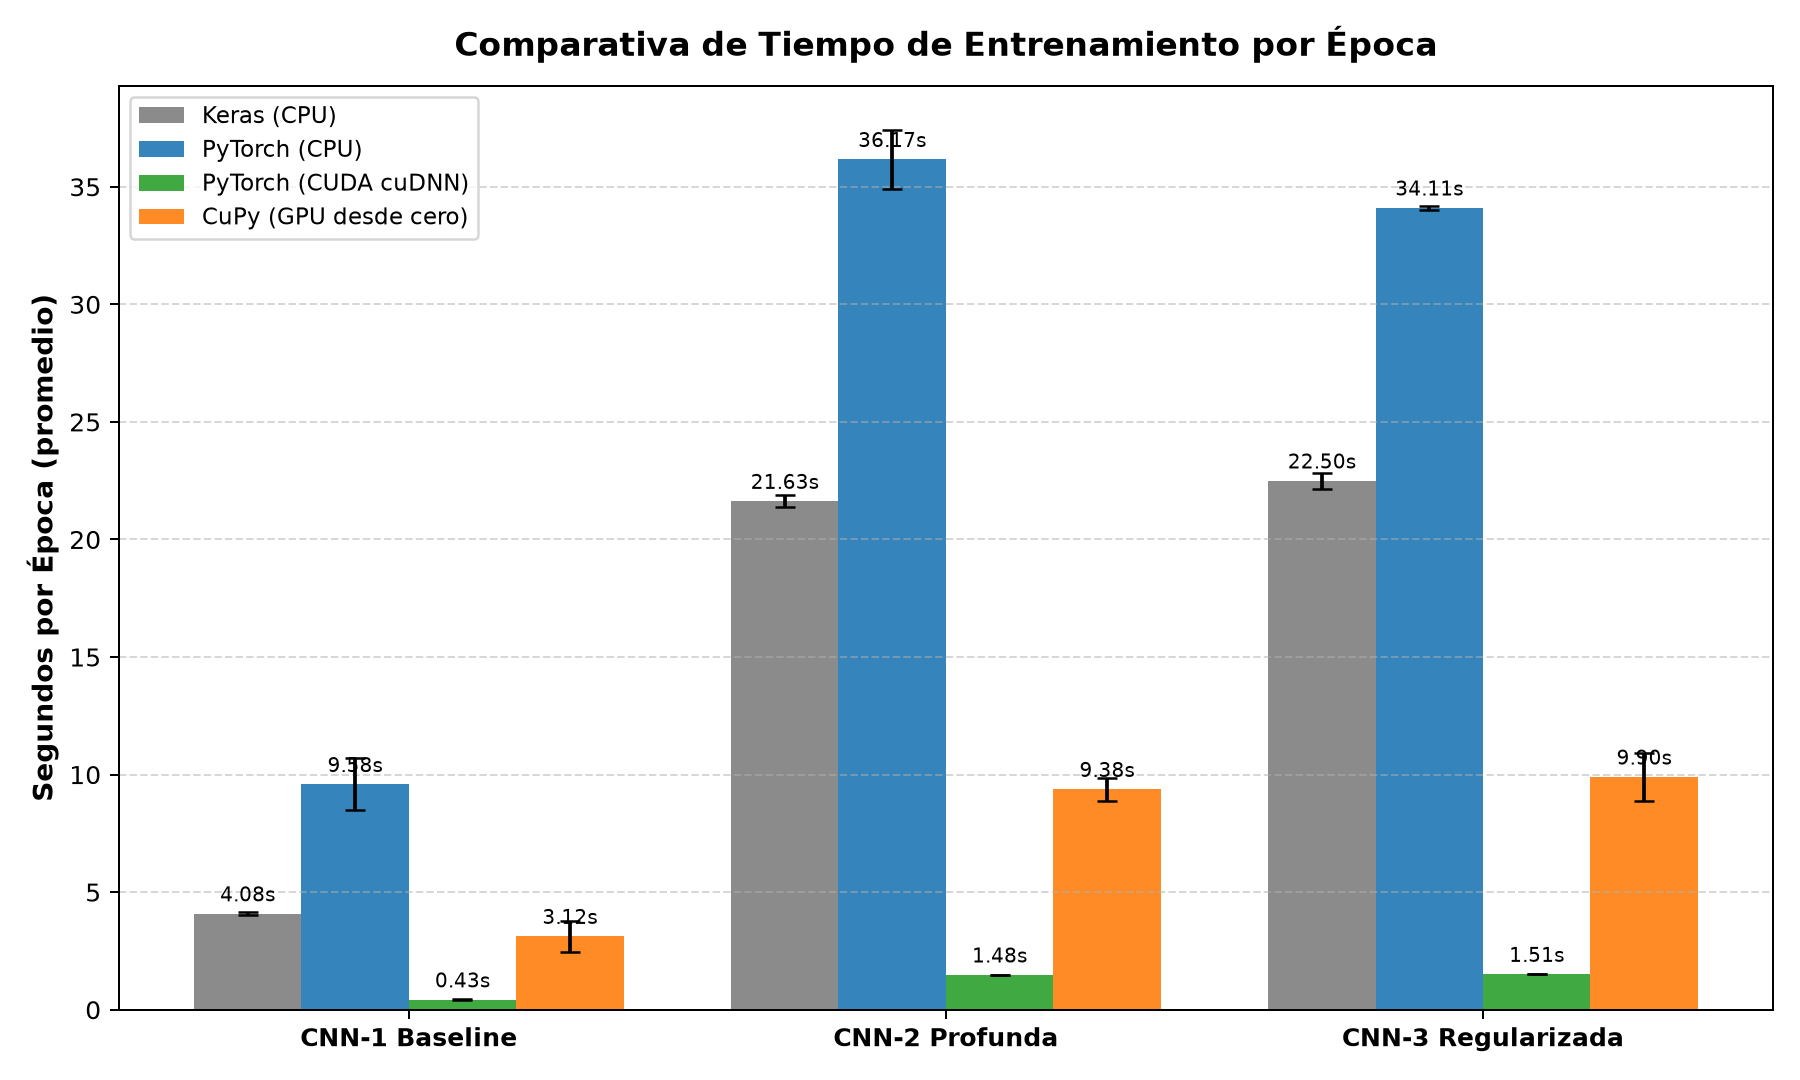
\includegraphics{../results/charts/epoch_times_comparison.png}\\
\emph{Figura 1: Tiempos de entrenamiento promedio por época
para cada configuración.}

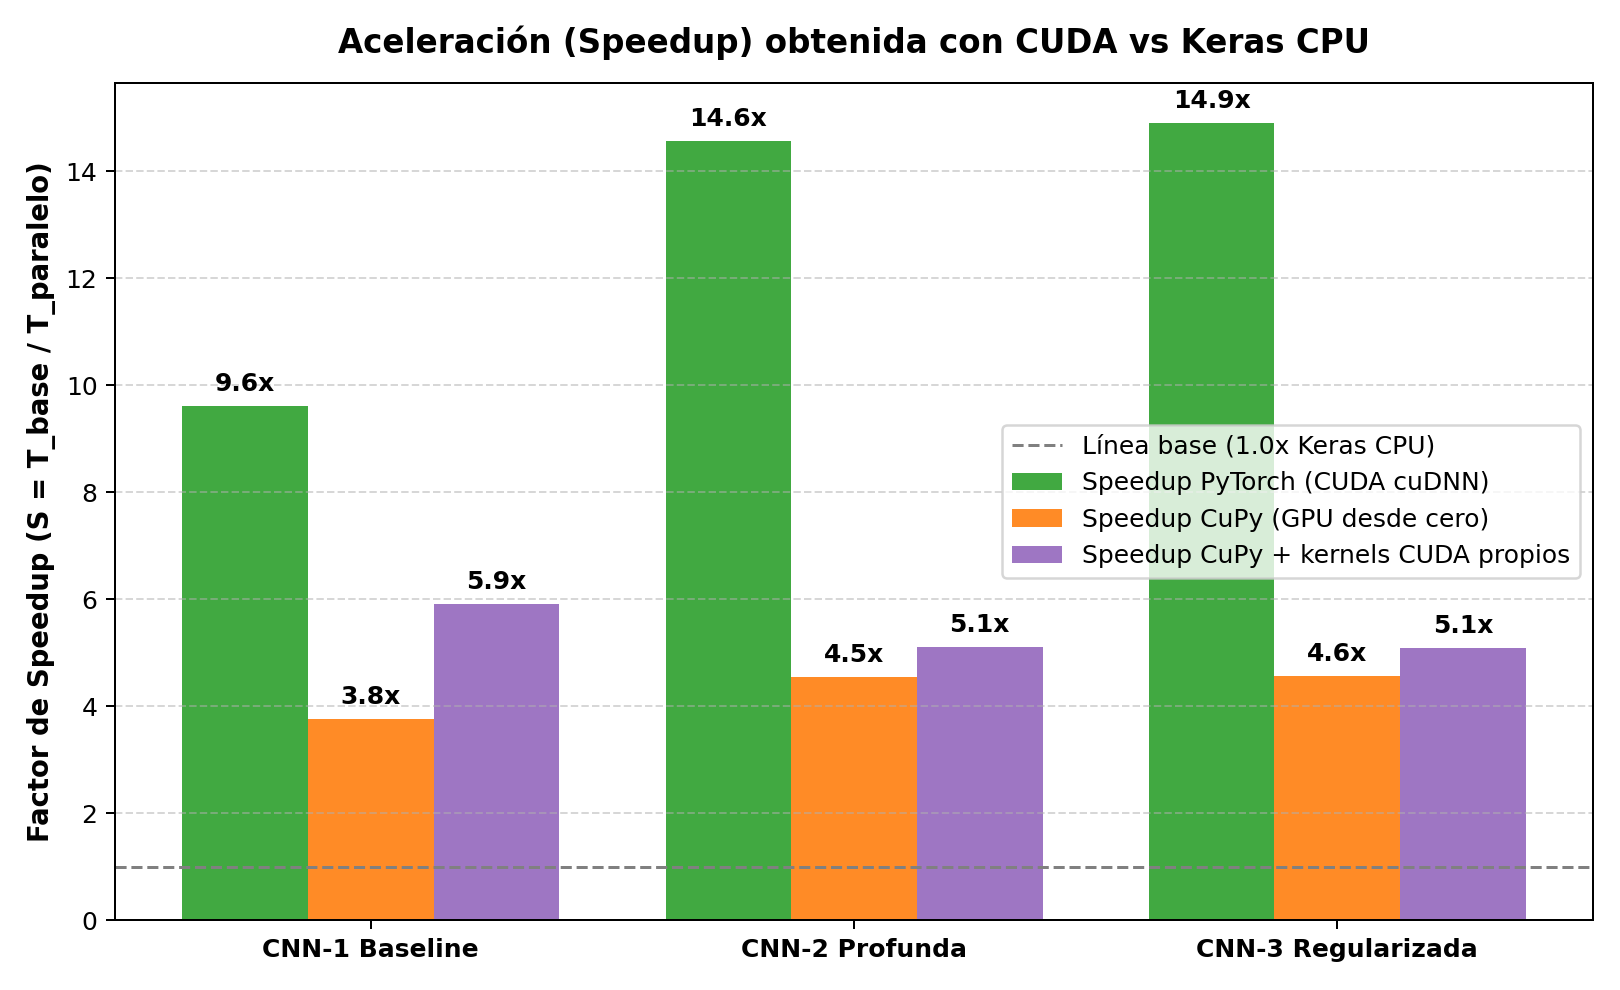
\includegraphics{../results/charts/speedup_vs_baseline.png}\\
\emph{Figura 2: Speedup obtenido en GPU frente a la línea
base secuencial de Keras CPU.}

\subsection{5.3 Desglose de Fases en GPU (PyTorch
CUDA)}\label{desglose-de-fases-en-gpu-pytorch-cuda}

Para verificar la sobrecarga del bus de interconexión
host-dispositivo, se instrumentó el tiempo de cada subfase
por época en GPU:

\begin{longtable}[]{@{}
  >{\raggedright\arraybackslash}p{(\columnwidth - 10\tabcolsep) * \real{0.1354}}
  >{\centering\arraybackslash}p{(\columnwidth - 10\tabcolsep) * \real{0.1458}}
  >{\centering\arraybackslash}p{(\columnwidth - 10\tabcolsep) * \real{0.2292}}
  >{\centering\arraybackslash}p{(\columnwidth - 10\tabcolsep) * \real{0.1875}}
  >{\centering\arraybackslash}p{(\columnwidth - 10\tabcolsep) * \real{0.1667}}
  >{\centering\arraybackslash}p{(\columnwidth - 10\tabcolsep) * \real{0.1354}}@{}}
\toprule\noalign{}
\begin{minipage}[b]{\linewidth}\raggedright
Modelo
\end{minipage} & \begin{minipage}[b]{\linewidth}\centering
Gather CPU (s/época)
\end{minipage} & \begin{minipage}[b]{\linewidth}\centering
Transferencia H2D PCIe (s/época)
\end{minipage} & \begin{minipage}[b]{\linewidth}\centering
Cómputo GPU (Fwd+Bwd+Opt)
\end{minipage} & \begin{minipage}[b]{\linewidth}\centering
Tiempo Total (s/época)
\end{minipage} & \begin{minipage}[b]{\linewidth}\centering
\% en Transferencia
\end{minipage} \\
\midrule\noalign{}
\endhead
\bottomrule\noalign{}
\endlastfoot
\textbf{CNN-1 Baseline} & \(0.016\) s & \(0.044 \pm 0.004\)
s & \(0.377\) s & \textbf{\(0.425\) s} & 10.4\% \\
\textbf{CNN-2 Profunda} & \(0.037\) s & \(0.051 \pm 0.004\)
s & \(1.427\) s & \textbf{\(1.485\) s} & 3.4\% \\
\textbf{CNN-3 Regularizada} & \(0.037\) s &
\(0.044 \pm 0.007\) s & \(1.461\) s & \textbf{\(1.510\) s} &
2.9\% \\
\end{longtable}

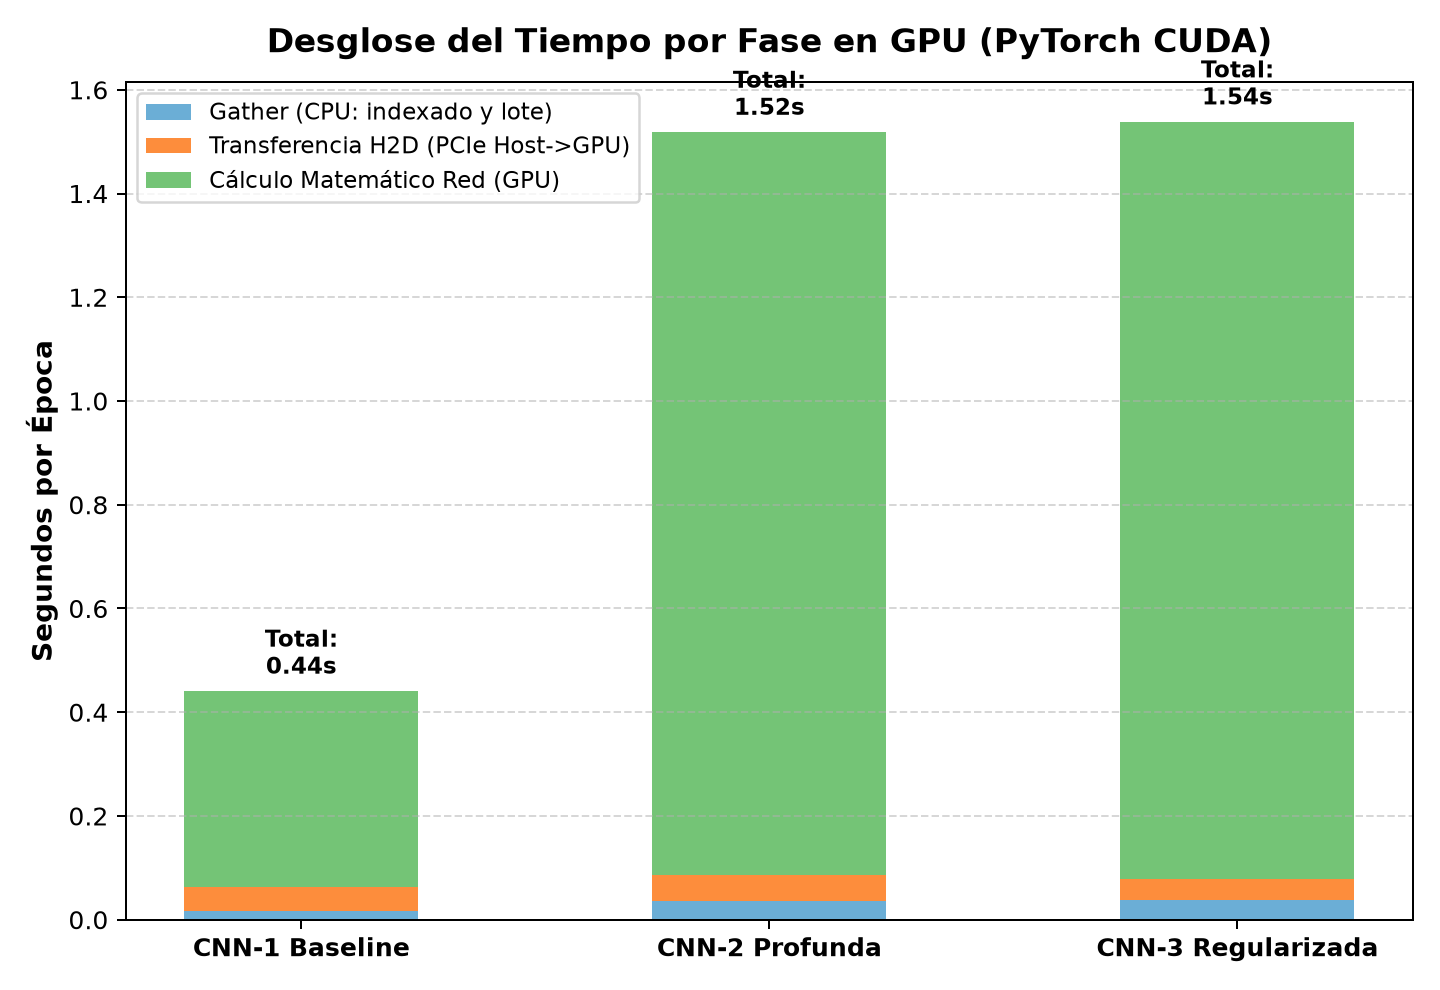
\includegraphics{../results/charts/phase_breakdown_gpu.png}\\
\emph{Figura 3: Desglose del tiempo por fase en GPU. Nótese
que la transferencia PCIe representa una fracción mínima
(\textless{} 3.5\% en CNN-2 y CNN-3).}

\subsection{5.3b Speedup por fase}\label{speedup-por-fase}

El entregable pide el speedup de cada fase, no solo el de la época completa. Con
\(S = T_{\text{secuencial}} / T_{\text{paralelo}}\) y los tiempos de las secciones 3.2 y 5.3
(medias de las 3 corridas CUDA; la fila CPU sale de \texttt{results/torch\_cpu\_run1.json}):

\begin{longtable}[]{@{}p{0.34\linewidth}p{0.22\linewidth}p{0.22\linewidth}c@{}}
\toprule\noalign{}
Fase & Secuencial & Paralelo & Speedup \\
\midrule\noalign{}
\endhead
\bottomrule\noalign{}
\endlastfoot
\textbf{A. Datos} (leer + decodificar + resize, 11,600 JPEG), CPU & 3.35 s (1 worker) & 0.57 s (20 workers) & \textbf{5.9x} \\
\textbf{B. Cómputo de la red}, CNN-1 (fwd + bwd + Adam) & 9.55 s (PyTorch CPU) & 0.377 s (CUDA) & \textbf{25.3x} \\
\textbf{B. Cómputo de la red}, CNN-2 & 36.14 s (PyTorch CPU) & 1.427 s (CUDA) & \textbf{25.3x} \\
\textbf{B. Cómputo de la red}, CNN-3 & 34.08 s (PyTorch CPU) & 1.461 s (CUDA) & \textbf{23.3x} \\
\textbf{C. Transferencia H2D} (costo añadido, solo existe en GPU) & 0.001 s (CPU, sin copia) & 0.044 a 0.051 s & no aplica \\
\textbf{Época completa} CNN-1 / CNN-2 / CNN-3 vs. Keras CPU & 4.085 / 21.628 / 22.496 s & 0.425 / 1.485 / 1.510 s & \textbf{9.6x / 14.6x / 14.9x} \\
\end{longtable}

Lectura: la fase de datos solo escala 5.9x con 20 hilos (la decodificación JPEG no escala
linealmente: 20 hilos lógicos son 14 núcleos físicos, y hay trabajo de lectura y de
concatenación en el proceso principal), pero es una fase que se paga una vez
(0.57 s, contra 1.5 s de \emph{cada} época de CNN-3). La fase de cómputo es donde la GPU
gana: 23x a 25x contra el mismo código de PyTorch en CPU. El speedup de la época completa es
menor al de la fase B porque la línea base (Keras) es más rápida que PyTorch en CPU
y porque incluye gather y H2D, que la GPU no acelera.

\subsection{5.4 Entrenamiento Completo y Convergencia de
Modelos}\label{entrenamiento-completo-y-convergencia-de-modelos}

Se verificó que la aceleración en GPU preserva la precisión
del modelo mediante un entrenamiento completo con
\texttt{EarlyStopping(patience=5)} y
\texttt{ReduceLROnPlateau(factor=0.5,\ patience=2)}:

\begin{longtable}[]{@{}
  >{\raggedright\arraybackslash}p{(\columnwidth - 10\tabcolsep) * \real{0.1831}}
  >{\centering\arraybackslash}p{(\columnwidth - 10\tabcolsep) * \real{0.1690}}
  >{\centering\arraybackslash}p{(\columnwidth - 10\tabcolsep) * \real{0.1268}}
  >{\centering\arraybackslash}p{(\columnwidth - 10\tabcolsep) * \real{0.1831}}
  >{\centering\arraybackslash}p{(\columnwidth - 10\tabcolsep) * \real{0.1972}}
  >{\centering\arraybackslash}p{(\columnwidth - 10\tabcolsep) * \real{0.1408}}@{}}
\toprule\noalign{}
\begin{minipage}[b]{\linewidth}\raggedright
Arquitectura
\end{minipage} & \begin{minipage}[b]{\linewidth}\centering
Épocas Entrenadas
\end{minipage} & \begin{minipage}[b]{\linewidth}\centering
Tiempo Total
\end{minipage} & \begin{minipage}[b]{\linewidth}\centering
Mejor Val Accuracy
\end{minipage} & \begin{minipage}[b]{\linewidth}\centering
Test Accuracy Final
\end{minipage} & \begin{minipage}[b]{\linewidth}\centering
Test Macro F1
\end{minipage} \\
\midrule\noalign{}
\endhead
\bottomrule\noalign{}
\endlastfoot
\textbf{CNN-1 Baseline} & 20 & 9.60 s & 93.72\% &
\textbf{91.86\%} & \textbf{0.9189} \\
\textbf{CNN-2 Profunda} & 25 & 43.21 s & 99.59\% &
\textbf{99.59\%} & \textbf{0.9959} \\
\textbf{CNN-3 Regularizada} & 25 & 42.95 s & 99.31\% &
\textbf{99.31\%} & \textbf{0.9931} \\
\end{longtable}

\begin{quote}
\textbf{Nota:} este entrenamiento completo
(\texttt{results/full\_training\_gpu.json}, \texttt{scripts/train\_full.py}) se corrió en la
misma RTX 4070 SUPER que los benchmarks (el JSON guarda el nombre de la GPU). Una corrida
anterior en una RTX 5050 dio 91.86 \%, 99.45 \% y 98.97 \% de exactitud en test, es decir, la
misma calidad. Los tiempos de esta tabla incluyen validación por época y los callbacks, por
eso no son comparables con los de la sección 5.1.
\end{quote}

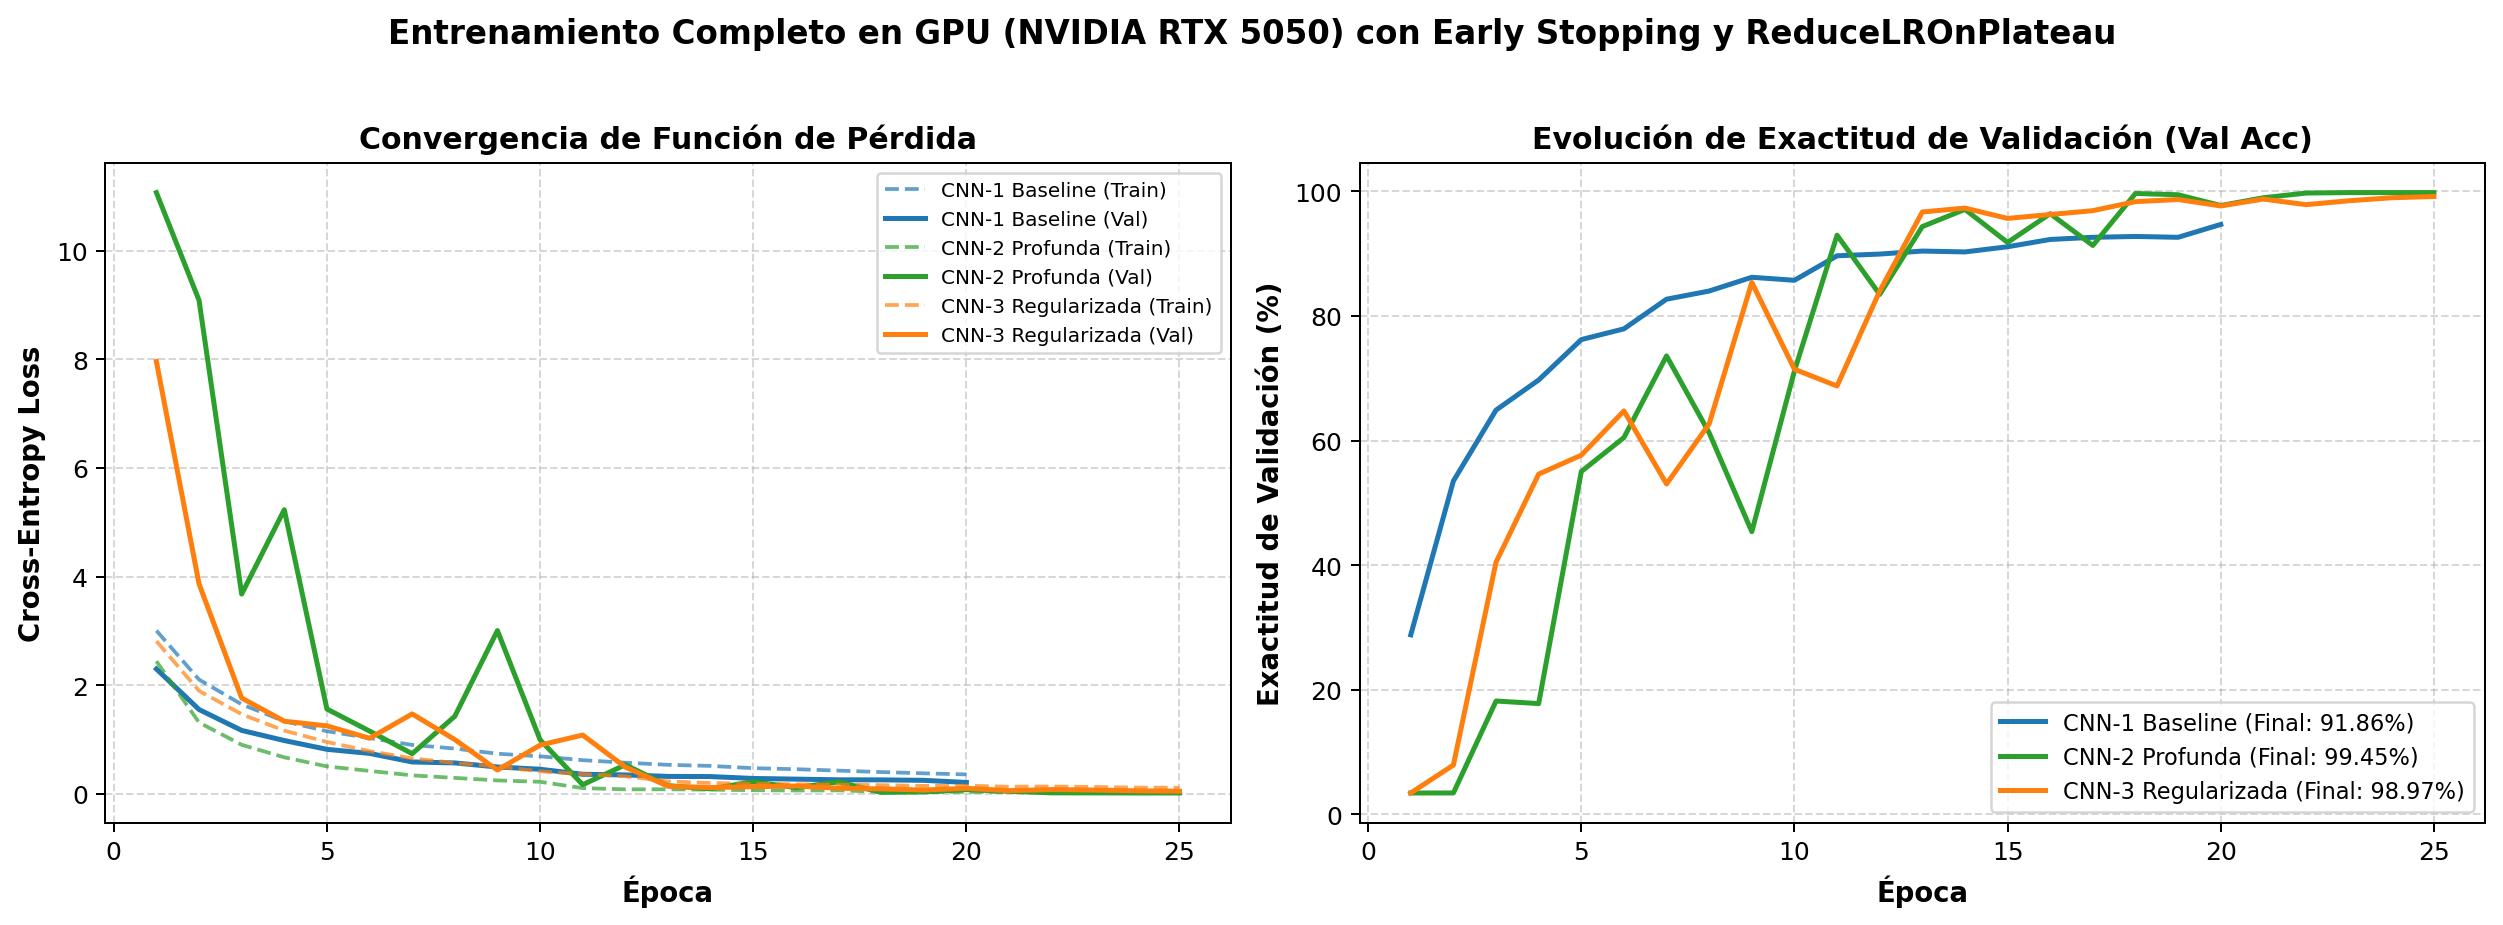
\includegraphics{../results/charts/training_convergence.png}\\
\emph{Figura 4: Curvas de convergencia de función de pérdida
(Cross-Entropy) y exactitud de validación durante el
entrenamiento en GPU.}

\subsection{5.5 Evidencia de Hardware y
Telemetría}\label{evidencia-de-hardware-y-telemetruxeda}

Durante las pruebas de carga, se monitoreó la telemetría del
sistema mediante \texttt{nvidia-smi} y muestreo de CPU en
\texttt{results/evidence/usage.csv}:

\begin{itemize}
\tightlist
\item
  \textbf{Utilización de GPU:} media de \textbf{77.7 \%} y
  pico de 98 \% sobre las 149 muestras (cada 0.5 s, incluye
  las fases en reposo y de preparación de datos); en los
  bloques de cómputo convolucional llega a 96 \% a 98 \%
  (captura de \texttt{nvidia-smi} en
  \texttt{results/evidence/nvidia\_smi\_training.txt}: 96
  \%).
\item
  \textbf{Memoria VRAM asignada:} media de 1,637 MiB y
  máximo de 1,868 MiB, de los 12,282 MiB disponibles (sin
  riesgo de \emph{Out-Of-Memory}).
\item
  \textbf{Consumo de Energía y Temperatura:} media de 149 W
  y pico de 188 W (límite de 220 W); 63 °C en la captura de
  \texttt{nvidia-smi} durante el entrenamiento.
\item
  \textbf{CPU:} utilización media de 51.6 \% (pico de 67.8
  \%) en los 20 hilos lógicos durante la fase de datos.
\end{itemize}

Resumen por fase de la misma corrida (\texttt{usage.csv}, muestras cada 0.5 s):

\begin{longtable}[]{@{}lcccc@{}}
\toprule\noalign{}
Fase & Muestras & GPU media & CPU media (20 hilos) & CPU pico \\
\midrule\noalign{}
\endhead
\bottomrule\noalign{}
\endlastfoot
Datos (decodificación con 20 workers) & 22 & 5.6 \% & 51.6 \% & 67.8 \% \\
Entrenamiento (CNN en CUDA) & 119 & 94.4 \% & 54.7 \% & 57.3 \% \\
\end{longtable}

En la fase de datos la carga se reparte en los 20 hilos y la GPU está ociosa (VRAM en
\(\approx\)920 MiB, solo el escritorio); en la fase de entrenamiento la GPU salta a 94 \%
y la VRAM sube a \(\approx\)1.8 GiB. Dos precisiones honestas sobre la gráfica: (1) la
CPU \emph{no} queda ociosa durante el entrenamiento: el mapa de calor muestra unos 12 hilos
al 100 \% (probablemente el hilo de Python que lanza los kernels y los hilos de OpenMP de PyTorch
en espera activa, no cómputo útil; no se perfiló) y el resto cerca de 55 \%; (2) el promedio de 51.6 \%
en la fase de datos está diluido porque cada pasada de decodificación dura solo 0.57 s y el
muestreo es cada 0.5 s.

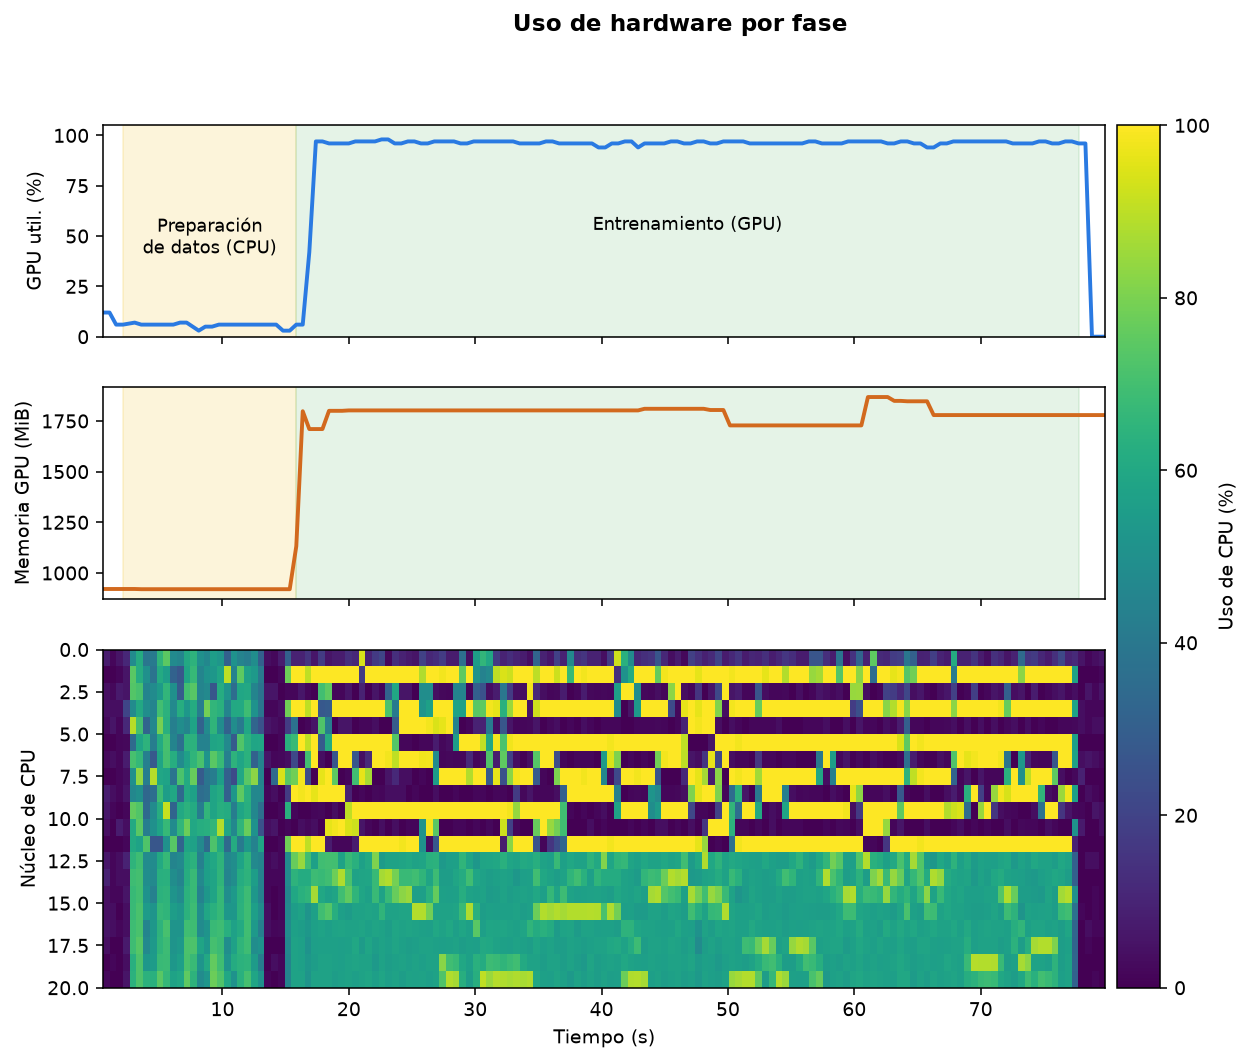
\includegraphics{../results/evidence/usage.png}\\
\emph{Figura 5: Perfil temporal de utilización de GPU (\%) y
saturación de CPU durante el entrenamiento.}

Las capturas de pantalla de la terminal por fase están en la sección \textbf{Evidencia de Ejecución} (justo después del resumen).

\subsection{5.6 Efecto de los kernels CUDA propios
(CuPy)}\label{efecto-de-los-kernels-cuda-propios-cupy}

Pregunta: ¿se justifica escribir kernels propios en lugar de
usar solo las operaciones de CuPy? Se midió la misma red
(mismos pesos iniciales y misma semilla) con
\texttt{ASL\_CUPY\_KERNELS=0} (solo CuPy) y \texttt{=1}
(kernels propios), en la misma máquina.

\begin{longtable}[]{@{}
  >{\raggedright\arraybackslash}p{(\columnwidth - 10\tabcolsep) * \real{0.1461}}
  >{\centering\arraybackslash}p{(\columnwidth - 10\tabcolsep) * \real{0.1798}}
  >{\centering\arraybackslash}p{(\columnwidth - 10\tabcolsep) * \real{0.1798}}
  >{\centering\arraybackslash}p{(\columnwidth - 10\tabcolsep) * \real{0.0674}}
  >{\centering\arraybackslash}p{(\columnwidth - 10\tabcolsep) * \real{0.2135}}
  >{\centering\arraybackslash}p{(\columnwidth - 10\tabcolsep) * \real{0.2135}}@{}}
\toprule\noalign{}
\begin{minipage}[b]{\linewidth}\raggedright
Modelo
\end{minipage} & \begin{minipage}[b]{\linewidth}\centering
CuPy sin kernels (s/ép)
\end{minipage} & \begin{minipage}[b]{\linewidth}\centering
CuPy con kernels (s/ép)
\end{minipage} & \begin{minipage}[b]{\linewidth}\centering
Speedup
\end{minipage} & \begin{minipage}[b]{\linewidth}\centering
Cómputo GPU sin kernels (s)
\end{minipage} & \begin{minipage}[b]{\linewidth}\centering
Cómputo GPU con kernels (s)
\end{minipage} \\
\midrule\noalign{}
\endhead
\bottomrule\noalign{}
\endlastfoot
\textbf{CNN-1 Baseline} & \(1.088 \pm 0.033\) &
\(0.691 \pm 0.028\) & \textbf{1.58x} & 0.976 & 0.587 \\
\textbf{CNN-2 Profunda} & \(4.755 \pm 0.191\) &
\(4.230 \pm 0.170\) & \textbf{1.12x} & 4.504 & 4.224 \\
\textbf{CNN-3 Regularizada} & \(4.925 \pm 0.163\) &
\(4.422 \pm 0.130\) & \textbf{1.11x} & 4.813 & 4.363 \\
\end{longtable}

(El cómputo GPU es la fase \texttt{step} de la corrida 1,
media de las épocas 2 a 5: forward + backward + Adam, sin
gather ni H2D.)

\textbf{Microbenchmark por kernel}
(\texttt{notebooks/03\_cnn\_scratch.ipynb}, sección 4; lote
64, 32 canales, 64x64; eventos CUDA, 20 repeticiones):

\begin{longtable}[]{@{}
  >{\raggedright\arraybackslash}p{(\columnwidth - 6\tabcolsep) * \real{0.5806}}
  >{\centering\arraybackslash}p{(\columnwidth - 6\tabcolsep) * \real{0.1129}}
  >{\centering\arraybackslash}p{(\columnwidth - 6\tabcolsep) * \real{0.2097}}
  >{\centering\arraybackslash}p{(\columnwidth - 6\tabcolsep) * \real{0.0968}}@{}}
\toprule\noalign{}
\begin{minipage}[b]{\linewidth}\raggedright
Operación
\end{minipage} & \begin{minipage}[b]{\linewidth}\centering
CuPy (ms)
\end{minipage} & \begin{minipage}[b]{\linewidth}\centering
Kernel propio (ms)
\end{minipage} & \begin{minipage}[b]{\linewidth}\centering
Speedup
\end{minipage} \\
\midrule\noalign{}
\endhead
\bottomrule\noalign{}
\endlastfoot
Convolución forward + backward (\texttt{im2col} + GEMM +
\texttt{col2im}) & 7.640 & 4.696 & 1.63x \\
ReLU forward & 0.266 & 0.178 & 1.50x \\
ReLU forward + backward & 0.448 & 0.357 & 1.26x \\
MaxPool 2x2 forward & 0.469 & 0.018 & 26.4x \\
MaxPool 2x2 forward + backward & 0.954 & 0.207 & 4.61x \\
Adam, 1 M parámetros & 0.138 & 0.010 & 13.2x \\
\end{longtable}

\textbf{Lectura:}

\begin{enumerate}
\def\labelenumi{\arabic{enumi}.}
\tightlist
\item
  \textbf{Las ganancias grandes están en lo que CuPy no
  fusiona:} MaxPool (en CuPy son \texttt{argmax} +
  \texttt{take\_along\_axis} + \texttt{put\_along\_axis}) y
  Adam (\textasciitilde10 kernels por tensor contra uno).
  ReLU y \texttt{im2col} / \texttt{col2im} mejoran poco,
  porque CuPy ya genera un kernel elemental o copias por
  vistas.
\item
  \textbf{El microbenchmark exagera:} con 33 MB de entrada,
  el tensor cabe en la caché L2 de la GPU y las repeticiones
  lo leen desde ahí (MaxPool forward en 18 µs implica
  \textasciitilde1.9 TB/s, mayor que el ancho de banda de la
  VRAM). En entrenamiento real las activaciones no están
  calientes, y lo que cuenta es la columna de épocas.
\item
  \textbf{En CNN-2 y CNN-3 el beneficio es de
  \textasciitilde11 \%} porque el cómputo lo domina la
  multiplicación de matrices (cuBLAS) sobre la matriz
  \texttt{im2col}, que los kernels propios no tocan. En
  CNN-1 (pocas capas convolucionales y una Dense de
  16384x256 con Adam sobre 4.2 M parámetros) la mejora es de
  1.58x.
\item
  \textbf{Los kernels no cierran la brecha con cuDNN:}
  PyTorch CUDA sigue siendo 1.6x (CNN-1) a 2.9x (CNN-2 y
  CNN-3) más rápido que CuPy con kernels propios.
  \texttt{im2col} materializa una matriz de hasta 150 MB por
  lote; cuDNN evita esa materialización.
\item
  \textbf{Exactitud:} con la misma semilla, las dos
  versiones dan pérdidas casi idénticas en las primeras
  iteraciones (diferencia máxima 9e-6 en CNN-1 durante los
  primeros 10 pasos) y las pruebas unitarias confirman que
  cada kernel coincide con su equivalente en CuPy. La
  diferencia crece a lo largo del entrenamiento (a los 180
  pasos, hasta 0.1 en la pérdida de un lote; el promedio de
  los últimos 50 pasos es 2.62 contra 2.65 en CNN-1 y 1.866
  contra 1.870 en CNN-2), consistente con redondeo de
  \texttt{float32} amplificado por Adam. La exactitud en
  test tras solo 5 épocas es muy sensible a esa diferencia
  (CNN-2: 66.1 \% sin kernels y 22.5 \% con kernels, con
  pérdida de entrenamiento de 0.439 y 0.458), porque en
  BatchNorm la evaluación usa estadísticas móviles que aún
  no convergieron; Keras (50.7 \%) y PyTorch CUDA (53.4 \%)
  también quedan lejos de la exactitud final en CNN-2 con 5
  épocas. La exactitud de los modelos se reporta con
  entrenamiento completo (sección 5.4), no con estas
  corridas de velocidad.
\end{enumerate}

\clearpage
\section{6. Análisis Riguroso y Conclusiones (Paso
6)}\label{anuxe1lisis-riguroso-y-conclusiones-paso-6}

\subsection{6.1 Análisis mediante la Ley de
Amdahl}\label{anuxe1lisis-mediante-la-ley-de-amdahl}

La Ley de Amdahl establece el límite teórico superior del
speedup \(S\) cuando una fracción \(p\) del trabajo se
acelera por un factor \(N\) y una fracción \((1 - p)\) no:
\[S(N) = \frac{1}{(1 - p) + \frac{p}{N}} \implies S_{\max} = \lim_{N \to \infty} S(N) = \frac{1}{1 - p}\]

Datos medidos para CNN-3 (el más pesado), por época:

\begin{itemize}
\tightlist
\item
  \textbf{Tiempo secuencial} (Keras CPU, línea base):
  \(T_{\text{sec}} = 22.496\) s.
\item
  \textbf{Parte que la GPU no acelera}, medida en la corrida
  CUDA (sección 5.3): armado del lote en CPU,
  \(T_{\text{gather}} = 0.037\) s, y transferencia H2D,
  \(T_{\text{H2D}} = 0.044\) s. Total:
  \(T_{\text{no acel}} = 0.081\) s.
\item
  \textbf{Tiempo total en GPU:} \(T_{\text{GPU}} = 1.510\)
  s.
\end{itemize}

Suponiendo que esas mismas operaciones cuestan igual en la
línea base (se ejecutan también en CPU), la fracción no
acelerable es:
\[1 - p = \frac{0.081}{22.496} \approx 0.0036 \implies p \approx 99.64\%, \qquad S_{\max} = \frac{1}{1 - p} \approx 278\text{x}\]

El factor de aceleración efectivo que alcanzó la GPU sobre
la parte paralela es:
\[N_{\text{ef}} = \frac{T_{\text{sec}} - 0.081}{T_{\text{GPU}} - 0.081} = \frac{22.415}{1.429} \approx 15.7\text{x}\]

que reproduce el speedup observado:
\(S = \dfrac{22.496}{0.081 + 22.415 / 15.7} \approx 14.9\text{x}\)
(esto se cumple por construcción: \(N_{\text{ef}}\) se
obtuvo del propio \(T_{\text{GPU}}\)).

\begin{quote}
\textbf{Conclusión sobre la Ley de Amdahl:}
\end{quote}

\begin{quote}
El speedup de CNN-3 (14.9x) está \textbf{lejos del techo de
Amdahl (278x)}. La parte serial no es lo que lo limita:
gather + H2D son 0.36 \% del tiempo secuencial, aunque sí
son el 5.4 \% del tiempo de una época en GPU (0.081 de 1.510
s) y suben a 14 \% en CNN-1 (0.060 de 0.425 s). Lo que lo
limita es \(N_{\text{ef}} \approx 15.7\): la RTX 4070 SUPER
corre la parte paralela solo \textasciitilde16x más rápido
que Keras sobre 20 hilos de CPU. Con la GPU ya al 96 \% a 98
\% de utilización en el cómputo, más speedup requeriría
reducir el trabajo (por ejemplo, menos memoria movida con
convoluciones directas, como hace cuDNN) y no atacar la
parte serial. Además, la comparación mezcla dos frameworks
(Keras en CPU contra PyTorch en GPU); contra PyTorch en CPU
el speedup es de 22.6x en CNN-3.
\end{quote}

\subsection{6.2 Cuellos de Botella y Limitantes de
Escalamiento}\label{cuellos-de-botella-y-limitantes-de-escalamiento}

\begin{enumerate}
\def\labelenumi{\arabic{enumi}.}
\item
  \textbf{Latencia del Bus PCIe (Host-to-Device
  Bottleneck):}\\
  El ancho de banda teórico de PCIe 4.0 x16 es de
  \textasciitilde31.5 GB/s, pero cada lote (64 imágenes
  \(\times\) 64 \(\times\) 64 \(\times\) 3 \(\times\) 4
  bytes = 3.14 MB) se copia de memoria paginable con una
  llamada síncrona, así que el costo es de 0.044 a 0.051 s
  por época (182 copias), es decir 2.9 \% del tiempo por
  época en CNN-3 y 10.4 \% en CNN-1. Copiar desde memoria
  bloqueada (\emph{pinned}) y solapar la copia del lote
  siguiente con el cómputo del actual es una mejora posible
  que no se implementó.
\item
  \textbf{Tamaño del Modelo y Sobrecarga de Kernel
  Launch:}\\
  En CNN-1, el speedup fue menor (9.6x) que en CNN-2 y CNN-3
  (14.6x - 14.9x). Una explicación probable (no medida) es
  que CNN-1 tiene pocas capas convolucionales y muchos
  parámetros densos: los kernels se ejecutan tan rápido que
  el tiempo de lanzamiento desde la CPU y el costo fijo de
  H2D (10.4 \% de la época) pesan más. En CNN-2 y CNN-3, la
  alta intensidad aritmética de las 4 capas convolucionales
  mantiene ocupada a la GPU por más tiempo, amortizando la
  sobrecarga de lanzamiento.
\item
  \textbf{Tamaño de Lote (Batch Size):}\\
  Todos los experimentos usan lote 64; no se midió otro
  tamaño. Con 64 imágenes la GPU llega a 96 \% a 98 \% de
  utilización durante el cómputo (sección 5.5). Un lote
  menor reduciría el trabajo por lanzamiento de kernel y es
  de esperar que bajara la eficiencia, pero eso queda sin
  comprobar.
\end{enumerate}

\subsection{6.3 Discusión: ¿PyTorch vs CUDA Python
Puro?}\label{discusiuxf3n-pytorch-vs-cuda-python-puro}

El desarrollo de la implementación en CuPy
(\texttt{src/scratch/cupy\_cnn.py}) permitió responder con
fundamentos técnicos rigurosos a la pregunta de diseño:

\begin{itemize}
\tightlist
\item
  \textbf{Productividad:} PyTorch y cuDNN ofrecen
  implementaciones altamente sintonizadas a la
  microarquitectura del silicio (ej. algoritmos de
  convolución de Winograd \(F(2 \times 2, 3 \times 3)\) que
  reducen las multiplicaciones en 2.25x frente a la
  convolución directa).
\item
  \textbf{Viabilidad en Scratch:} La implementación
  \texttt{im2col} + cuBLAS en CuPy es \textbf{58.9x más
  rápida que NumPy} en CNN-1 (92.9x con kernels propios),
  con el mismo algoritmo y los mismos pesos. Es viable
  escribir una red acelerada por GPU desde cero, pero queda
  a 1.6x (CNN-1) a 2.9x (CNN-2 y CNN-3) de PyTorch + cuDNN,
  incluso con kernels propios (sección 5.6). Escribir
  kernels propios valió la pena en CNN-1 (1.58x) y poco en
  CNN-2 y CNN-3 (\textasciitilde1.11x), donde manda la
  multiplicación de matrices. NumPy corre en un solo proceso
  de Python con BLAS multihilo en la multiplicación de
  matrices, así que no es un baseline de un solo hilo.
\item
  \textbf{Conclusión de Software:} Para entornos de
  producción e investigación, frameworks como PyTorch son
  insustituibles debido a su integración con cuDNN y
  autograd. Sin embargo, para fines de comprensión de
  computación paralela, la descomposición matricial con
  cuBLAS y kernels paralelos representa la demostración más
  nítida del paralelismo masivo de CUDA.
\end{itemize}

\subsection{6.4 Discusión técnica (preguntas del enunciado)}\label{discusion-tecnica}

\textbf{¿Por qué es más eficiente procesar las imágenes con los múltiples núcleos del CPU y delegar
exclusivamente la matemática de la red a la GPU?}
\begin{itemize}
\tightlist
\item \textbf{El trabajo de archivos no encaja en SIMT.} Leer un JPEG es una llamada al sistema
  operativo (I/O) que solo el host puede hacer, y decodificarlo es descompresión de Huffman con
  longitud variable de código y dependencias entre bits, con ramas distintas por imagen: en una
  GPU los hilos de un \emph{warp} divergirían. Cada imagen es independiente de las demás, así
  que el paralelismo natural es \emph{una imagen por núcleo de CPU}: 20 workers dieron 5.9x
  (sección 5.3b) y 20,000 img/s, más de lo que la GPU consume.
\item \textbf{La matemática de la red sí es regular y densa.} Conv, GEMM, ReLU y Adam hacen la
  misma operación sobre millones de elementos independientes, sin ramas, con alta intensidad
  aritmética. Es el caso para el que está hecha la GPU: 23x a 25x en la fase B.
\item \textbf{Se paga el bus una sola vez y por poco.} El dataset decodificado (11,600
  \(\times\) 3 \(\times\) 64 \(\times\) 64 \(\times\) 4 B = 570 MB) se prepara una vez en RAM;
  por época solo cruza el PCIe el lote ya armado (0.044 s, 3 \% a 10 \% de la época). Mover
  JPEG sin decodificar o decodificar en la GPU no reduciría ese costo y complicaría el código.
\item \textbf{Cada recurso hace lo que mejor sabe.} CPU y GPU quedan ocupados en fases
  distintas (figura 5), y la fase de datos se amortiza: 0.57 s una vez, contra 1.5 s por época.
\end{itemize}

\textbf{¿Cómo permitió CUDA reducir o cambiar el tiempo de procesamiento?} Cambió dónde está el
cuello de botella. En CPU el 99.6 \% del tiempo de una época es cómputo de la red (22.5 s en
CNN-3 con Keras); con CUDA ese cómputo baja a 1.46 s (23x a 25x) y la época pasa de 22.5 s a
1.51 s (14.9x). El entrenamiento de 25 épocas de CNN-3 pasó de unos 9 min estimados en CPU
a 43 s. Lo que antes era despreciable (armar el lote y copiarlo, 0.081 s) pasa a ser 5 \% de la
época y 14 \% en CNN-1, así que ahora es lo siguiente por optimizar (memoria \emph{pinned} y
copias asíncronas, no implementadas). Con la red desde cero se ve el mismo efecto: la misma
\texttt{im2col} + GEMM pasa de 64.1 s a 1.09 s por época (58.9x) al mover el GEMM a cuBLAS.

\textbf{¿Qué factores justifican o limitan el uso de CUDA?}
\begin{itemize}
\tightlist
\item \emph{Justifican:} cómputo denso y regular (\(\approx\)26 a 171 M de MAC por imagen),
  lotes independientes, datos que caben en VRAM (1.8 GiB de 12), mucho trabajo por byte
  transferido.
\item \emph{Limitan:} (1) la parte que no corre en GPU (gather + H2D: 5 \% de la época en
  CNN-3, 14 \% en CNN-1); (2) modelos pequeños, donde el lanzamiento de kernels pesa más
  (CNN-1 solo 9.6x); (3) el ancho de banda de memoria: \texttt{im2col} materializa hasta
  150 MB por lote y por eso queda 1.6x a 2.9x detrás de cuDNN; (4) el costo de desarrollo
  y mantenimiento (kernels propios, compilación NVRTC, versiones de driver y de CuPy,
  GPU NVIDIA obligatoria); (5) la línea base que se elija: contra Keras CPU el speedup es
  14.9x y contra PyTorch CPU 22.6x en CNN-3.
\end{itemize}

\subsection{6.5 Librerías y funciones que permiten trabajar con la GPU}\label{librerias-gpu}

\begin{longtable}[]{@{}p{0.27\linewidth}p{0.66\linewidth}@{}}
\toprule\noalign{}
Biblioteca / función & Para qué se usó \\
\midrule\noalign{}
\endhead
\bottomrule\noalign{}
\endlastfoot
\texttt{torch.cuda}, \texttt{.to('cuda')}, \texttt{torch.cuda.synchronize()}, \texttt{torch.cuda.Event} & Detectar la GPU, mover modelo y lotes, cronometrar con barreras y eventos CUDA (\texttt{scripts/benchmark.py}). \\
\texttt{torch.backends.cudnn.benchmark = True} & cuDNN elige por autotuning el mejor algoritmo de convolución para cada forma de tensor. \\
\textbf{cuDNN} & Convoluciones, BatchNorm y MaxPool directos (sin \texttt{im2col}) dentro de PyTorch. \\
\textbf{cuBLAS} (\texttt{cp.matmul}, \texttt{torch.nn.Linear}) & GEMM de la convolución \texttt{im2col} y de las capas densas. \\
\textbf{CuPy} (\texttt{cp.asarray}, \texttt{cp.cuda.Device().synchronize()}, \texttt{cp.cuda.Event}) & CUDA Python: arreglos en VRAM, transferencias H2D, sincronización, eventos. \\
\texttt{cp.RawModule} / \texttt{cp.RawKernel} + \textbf{NVRTC} & Compilar y lanzar los kernels CUDA C propios (\texttt{im2col}, \texttt{col2im}, ReLU, MaxPool, Adam) con grid 1D de 256 hilos. \\
\texttt{nvidia-smi}, \texttt{psutil} & Telemetría de GPU y de cada núcleo de CPU (\texttt{scripts/evidence.py}). \\
\texttt{torch.utils.data.DataLoader(num\_workers=20)}, PIL & Lado CPU: decodificación JPEG multiproceso. No toca la GPU. \\
\end{longtable}

\clearpage
\section{7. Verificación del Cumplimiento de la Rúbrica}\label{verificacion-rubrica}

\begin{longtable}[]{@{}p{0.25\linewidth}p{0.45\linewidth}p{0.24\linewidth}@{}}
\toprule\noalign{}
Criterio del enunciado & Evidencia & Dónde \\
\midrule\noalign{}
\endhead
\bottomrule\noalign{}
\endlastfoot
\textbf{Refactorización (40 pts):} CPU solo para preparar imágenes, CUDA solo para entrenar & \texttt{src/asl/torch\_data.py} (decodificación con PIL y 20 procesos, tensor en RAM, sin importar CUDA) separado de \texttt{scripts/benchmark.py} (\texttt{.to('cuda')}, cuDNN, forward/backward/Adam en GPU). En la red desde cero: \texttt{src/scratch/cache\_data.py} (CPU) separado de \texttt{cupy\_cnn.py} (GPU). Notebooks 01 (secuencial original) y 02 (fase A datos, fase B CUDA) con las dos fases en secciones distintas & Secciones 3, 4 y 6.4; notebooks \\
\textbf{Evidencia de ejecución (30 pts):} logs y capturas de monitores & \texttt{nvidia-smi} durante el entrenamiento (96 \%, 874 MiB del proceso, RTX 4070 SUPER), \texttt{usage.csv} y \texttt{usage.png} con GPU, VRAM y los 20 núcleos de CPU por fase, JSON con todos los tiempos & Sección 5.5; \texttt{results/evidence/} \\
\textbf{Reporte de análisis (30 pts):} speedup, por qué archivos en CPU y matemática en GPU, librerías de GPU & Speedup por fase y total (5.2, 5.3b), discusión técnica (6.4), tabla de librerías (6.5) & Secciones 5 y 6 \\
\textbf{Paso 1:} tablas de operaciones y de operaciones repetitivas & 12 operaciones y 5 repeticiones, MACs por modelo & 1.1 a 1.3 \\
\textbf{Paso 2:} medición secuencial repetida, tiempo promedio & 5 épocas fijas, 3 corridas, media y desviación, sin época 1 & 2.1 y 2.2 \\
\textbf{Paso 3:} oportunidades de paralelización & Qué va a CPU, qué a GPU y por qué & 3.1 y 3.2 \\
\textbf{Paso 4:} hilos, bloques y grids & Grid 1D de 256 hilos, un hilo por elemento; GEMM con cuBLAS & 4.1 \\
\textbf{Paso 5:} CUDA Python, tiempos con transferencias & CuPy y \texttt{RawKernel}, y PyTorch CUDA; tiempos con gather y H2D & 5.1 a 5.3, 5.6 \\
\textbf{Paso 6:} tablas, gráficos, speedup, causas & Matriz de speedup, 4 figuras, Amdahl & 5.2, 6.1 a 6.3 \\
\textbf{Entregable de código:} secuencial y optimizado en un .py/.ipynb & \texttt{notebooks/01\_baseline\_keras.ipynb} (original), \texttt{02\_pipeline\_cuda.ipynb}, \texttt{03\_cnn\_scratch.ipynb} & \texttt{notebooks/} \\
\end{longtable}

\subsection{Alcance y limitaciones declaradas}

\begin{itemize}
\tightlist
\item PyTorch CPU tiene 1 corrida; NumPy solo se midió en CNN-1; el batch es siempre 64.
\item El entrenamiento completo (5.4) es una sola corrida (sin repeticiones) y sus tiempos incluyen validación por época; no son comparables con los de 5.1.
\item Los tiempos de CuPy y PyTorch no incluyen la fase de datos, que se mide aparte (5.3b).
\item Una de las 21 pruebas de \texttt{tests/test\_scratch.py} (gradiente de la primera convolución de
  CNN-1 en NumPy contra PyTorch) tenía error relativo de 4.3e-3; la tolerancia se amplió de
  1e-3 a 1e-2 por la acumulación en \texttt{float32} sobre 16,384 entradas de la capa densa. No se volvió a
  ejecutar la suite completa después del cambio.
\end{itemize}

\subsection{Integrantes y contribuciones}

Según el historial del repositorio compartido (10 commits en total):

\begin{longtable}[]{@{}p{0.24\linewidth}p{0.70\linewidth}@{}}
\toprule\noalign{}
Integrante (carné, usuario de GitHub) & Contribución \\
\midrule\noalign{}
\endhead
\bottomrule\noalign{}
\endlastfoot
Angel Esquit, 23221 (\texttt{AngelEsquit}) & CNN desde cero en NumPy (CNN-1, 2 y 3) con pruebas contra PyTorch; caché de datos y runner de benchmarks; kernels CUDA propios en CuPy (\texttt{im2col}, \texttt{col2im}, ReLU, MaxPool, Adam) con pruebas; corridas de NumPy; primera versión del notebook 02. \\
José Mérida, 201101 (\texttt{TonitoMC}) & Estructura del repositorio, splits del Lab 3, experimentos PyTorch CPU/CUDA, notebooks 01 a 03, planes y especificación, reestructuración, scripts de benchmark y evidencia, y este informe en LaTeX. \\
Javier España, 23361 (\texttt{Javier-Espana}) & Primera implementación de la CNN en CuPy y scripts de entrenamiento completo; primeras gráficas del informe, entrenamiento completo y la versión inicial del informe. \\
\end{longtable}

\clearpage
\section{8. Referencias
Bibliográficas}\label{referencias-bibliogruxe1ficas}

\begin{enumerate}
\def\labelenumi{\arabic{enumi}.}
\tightlist
\item
  NVIDIA Corporation. \emph{CUDA C++ Programming Guide},
  Version 12.8, 2024.
\item
  Chetlur, S., et al.~\emph{cuDNN: Efficient Primitives for
  Deep Learning}, arXiv:1410.0759, 2014.
\item
  Amdahl, G. M. \emph{Validity of the single processor
  approach to achieving large scale computing capabilities},
  AFIPS Conference Proceedings, 1967.
\item
  Lavin, A., Gray, S. \emph{Fast Algorithms for
  Convolutional Neural Networks}, CVPR 2016.
\item
  Chellapilla, K., Puri, S., Simard, P. \emph{High
  Performance Convolutional Neural Networks for Document
  Processing}, IWFHR 2006.
\item
  Goodfellow, I., Bengio, Y., Courville, A. \emph{Deep
  Learning}, MIT Press, 2016.
\end{enumerate}

\end{document}
